\documentclass{article}
\usepackage[english]{babel}
\usepackage[letterpaper,top=2cm,bottom=2cm,left=3cm,right=3cm,marginparwidth=1.75cm]{geometry}

% Useful packages
\usepackage{amsmath}
\usepackage{amsfonts}
\usepackage{graphicx}
\usepackage[colorlinks=true, allcolors=blue]{hyperref}
\usepackage{booktabs}
\usepackage{subcaption}
\usepackage{microtype}
% bibliography
\usepackage{authblk}
\usepackage{csquotes}
%\usepackage[style=numeric, backend=bibtex]{biblatex}
%\addbibresource{references.bib}
% tikz
\usepackage{tikz}
\usetikzlibrary{positioning, arrows.meta, fit, shapes.geometric, calc, shadows}
% notes
\usepackage{todonotes}
% To show the labels of sections, equations, figures, references, etc.
% \usepackage{showkeys}
% \renewcommand*\showkeyslabelformat[1]{%
%   \fbox{\parbox[t]{\marginparwidth}{\raggedright\normalfont\tiny\ttfamily#1}}}
% To do notes
\setlength{\marginparwidth}{2cm}
\newcommand{\mg}[1]{\todo[color=green!20]{\textbf{MG:} #1}}
\newcommand{\mgt}[1]{\todo[color=green!20, inline]{\textbf{MG:} #1}}
\newcommand{\mm}[1]{\todo[color=orange!20]{\textbf{MM:} #1}}
\newcommand{\mt}[1]{\todo[color=orange!20, inline]{\textbf{MM:} #1}}

% numeri di riga
\usepackage[switch]{lineno}

\title{A Geometry-Aware Isogeometric Neural Preconditioner for Partial Differential Equations}
\date{}
\author[1]{Massimiliano Ghiotto}
\author[2]{Matthias M\"oller}
\author[1]{Monica Montardini}
\author[1]{Giancarlo Sangalli}
\author[1]{Mattia Tani}
\affil[1]{Department of Mathematics, University of Pavia}
\affil[2]{Applied Mathematics, Delft University of Technology}

% User defined commands
\def\numpatch{\mathcal{N}_{patch}}
\newcommand{\ndof}{m}
\newcommand{\vect}[1]{\boldsymbol{#1}}
\newcommand{\R}{\mathbb{R}}
\newcommand{\N}{\mathbb{N}}
\newcommand{\Dlat}{d_v} % Latent dimension
\newcommand{\reflevel}{\ell} % Refinement level


% Theorem enviromentals
% theorems and similar stuff
\usepackage{amsthm}
\theoremstyle{plain}
\newtheorem{ass}{Assumption} 
\newtheorem{lemma}{Lemma}
\newtheorem{prop}{Proposition}
\newtheorem{theorem}{Theorem}
\newtheorem{df}{Definition}
\newtheorem{rmk}{Remark}
\newtheorem{cor}{Corollary}
\numberwithin{equation}{section}


\begin{document}
\maketitle
% \tableofcontents
\linenumbers
%%%%%%%%%%%%%%%%%%%%%%%%%%%%%%%%%%%%%%%%%
%% Abstract 
%%%%%%%%%%%%%%%%%%%%%%%%%%%%%%%%%%%%%%%%%
\begin{abstract}
    We propose a geometry-aware preconditioning framework for Isogeometric Analysis based on Isogeometric Neural Networks (IgaNets). The method embeds a trained IgaNet as a coarse-grid corrector within a two-level multigrid V-cycle, combining classical smoothers (Jacobi, Gauss-Seidel, and Fast Diagonalization) with a neural network based correction that targets the low-frequency error components that classical smoothers struggle to reduce. The multilevel structure allows a single IgaNet, trained at a coarse discretization, to precondition problems at finer mesh refinements and higher polynomial degrees without retraining. To handle both fixed and variable computational domains, we introduce a Transformer-based IgaNet architecture that encodes the spline control points of the geometry through self-attention layers and outputs a linear operator acting on the discretized forcing term, thereby preserving the linearity of the solution map and enabling the use of standard Krylov methods. Extensive numerical experiments demonstrate that the proposed preconditioners consistently reduce the iteration count of Krylov solvers, generalizing effectively across varying source terms, geometric domains, mesh sizes, and polynomial degrees, including unseen geometries and out-of-distribution data.
\end{abstract}

%%%%%%%%%%%%%%%%%%%%%%%%%%%%%%%%%%%%%%%%%
%% Section: introduction
%%%%%%%%%%%%%%%%%%%%%%%%%%%%%%%%%%%%%%%%%
\section{Introduction} \label{sec:introduction}
Partial Differential Equations (PDEs) are the mathematical backbone for modeling physical phenomena across a wide spectrum of scientific and engineering disciplines.
%In contexts such as optimal design, uncertainty quantification, and inverse analysis, these equations frequently arise in a parametric setting, necessitating the evaluation of the solution map for a multitude of input configurations. These configurations range from material coefficients and source terms to boundary conditions and geometric domains.
To approximate the solutions of PDEs with high fidelity, Isogeometric Analysis (IGA)~\cite{hughes2005isogeometric} has emerged as a powerful discretization paradigm. By adopting Non-Uniform Rational B-Splines (NURBS) or other CAD-compatible spline bases as the ansatz functions for the analysis, IGA bridges the gap between geometric design and numerical simulation, offering exact geometric representation and superior approximation properties compared to standard Finite Element Methods.

However, the advantages of IGA come at a computational cost. The discretization of elliptic  PDEs yields large-scale systems of linear equations, where the system matrix depends on the problem parameters. For high-resolution simulations, direct solvers become prohibitively expensive due to their computational complexity scaling. Consequently, iterative Krylov subspace methods, e.g., Generalized Minimal Residual (GMRES), Conjugate Gradient (CG), are the standard choice for large-scale problems. The efficacy of these solvers is intimately tied to the spectral properties of the system matrix; specifically, the convergence rate typically deteriorates as the condition number grows. Modeling complex geometries with IGA often requires mesh-refinement and degree-elevation, both of which adversely affect the condition number~\cite{sangalli2016isogeometric, gahalaut2019condition}.
To counteract this ill-conditioning, robust preconditioning strategies are indispensable. Classical approaches include stationary iterative methods such as Jacobi and Gauss-Seidel preconditioners \cite{van2003iterative}, which are effective at dampening high-frequency error modes, as well as multigrid methods \cite{trottenberg2000multigrid}, which address error components across multiple scales by combining smoothing iterations with coarse-grid corrections. 
%In the IGA context, the Fast Diagonalization method \cite{Lynch1964, sangalli2016isogeometric} exploits the tensor-product structure of B-spline discretizations.
\\
Recently, the Scientific Machine Learning community has explored Neural Operators (NOs) as a paradigm to approximate the solution operators coming from the PDEs. Distinct from classical neural networks that map finite-dimensional vectors, NOs learn mappings between infinite-dimensional function spaces. Prominent architectures include Fourier Neural Operators (FNOs,~\cite{li2021fourier}), which leverage the Fast Fourier Transform to efficiently parametrize integral kernels, and Deep Operator Networks (DeepONet,~\cite{lu2021learning}), which are based on the universal approximation theorem for operators~\cite{chen1995universal}. DeepONets have gained significant traction due to their flexibility; unlike FNOs which typically require uniform grid data, DeepONets utilize a dual-network structure that allows them to operate on arbitrary discretizations without modification.

Neural operators exhibit the so-called ``spectral bias'' \cite{rahaman2019spectral}: they learn low-frequency components of the target function rapidly while struggling to capture high-frequency details. As discussed above, classical preconditioners act as smoothers that efficiently damp high-frequency error modes but leave low-frequency components essentially untouched. This complementary spectral behavior suggests to embed a trained neural operator as a coarse-grid corrector within a classical iterative solver \cite{kopanivcakova2025deeponet, lee2025hybrid, karniadakis2025nonlinearprec, karniadakis2025nspod}.
Despite the growing work on neural operators as preconditioners, most existing architectures are designed for fixed geometric domains. A notable exception is represented by \cite{lee2025hybrid}, where a geometry-aware preconditioner is implemented.
Nevertheless, adapting to a variation in the computational domain typically necessitates a full retraining of the network, or a fine tune of it \cite{kahana2023geometry}, resulting in an inefficient approach for multi-geometry parametric studies.
In this work, we propose a novel, geometry-aware preconditioning framework tailored for isogeometric analysis. We introduce an architecture based on Isogeometric Neural Networks (\textbf{IgaNets}, \cite{moller2026iganet}), which intrinsically leverages the B-spline structure of the IGA discretization.
Specifically, we discretize the PDE and the geometric domain with B-spline basis; the control points of the geometry and the discretized right-hand side are then passed directly as input to the network. We validate the proposed architecture through extensive numerical experiments, first considering the source term as the sole parameter on a fixed geometry, and subsequently addressing the more general case where both the right-hand side and the computational domain vary.
This approach draws a parallel with Spectral Neural Operators \cite{fanaskov2023spectral}, where the network operates in the frequency domain of a specific basis. However, instead of relying on global Fourier or Chebyshev bases, we employ a spline basis. This allows us to represent and handle complex geometries effectively while preserving the exact geometric mapping inherent to the underlying PDE solver.

The novel main contributions of this paper are the following:
\begin{itemize}
    \item We develop a preconditioning strategy that synergizes IgaNets with classical preconditioners, in particular we combine IgaNets with Jacobi, Gauss-Seidel and Fast Diagonalization \cite{Lynch1964} methods.
    \item We propose a multilevel preconditioning strategy capable of operating across different mesh refinements and polynomial degrees using a single, fixed IgaNet model, thereby avoiding the computational cost of retraining. We rigorously analyze the method's computational performance, specifically investigating its robustness with respect to the discretization parameters.
    \item We introduce a novel transformer-based IgaNet architecture designed to handle variable geometric domains. By treating the geometric description as a sequence of tokens, this architecture allows a single and fixed model to generalize across a wide class of domains.
    \item We demonstrate through extensive numerical experiments that our combined preconditioning strategy reduces the iteration count of Krylov solvers. We initially evaluate the performance on a fixed geometry by varying only the source term, and subsequently extend the analysis to scenarios where both the right-hand side and the computational domain vary, exhibiting generalization capabilities to unseen geometries and source terms.
\end{itemize}

The remainder of the paper is detailed as follows. Section \ref{sec:preliminaries} outlines the mathematical preliminaries, including the fundamentals of IGA, the problem formulation and the preconditioning strategy. Section \ref{sec:experiments_fixed} presents the methodology and numerical experiments for fixed domains, focusing on varying source terms. Section \ref{sec:experiments_rhs_domain} extends the methodology to variable domains, introducing the transformer-based architecture and validating its performance on varying geometries. Finally, Section \ref{sec:conclusions} draws conclusions and discusses future research directions.

%%%%%%%%%%%%%%%%%%%%%%%%%%%%%%%%%%%%%%%%%
%% Section
%%%%%%%%%%%%%%%%%%%%%%%%%%%%%%%%%%%%%%%%%
\section{Preliminaries} \label{sec:preliminaries}

%%%%%%%%%%%%%%%%%%%%%%%%%%%%%%%%%%%%%%%%%
\subsection{B-splines} \label{subsec:prel-bsplines}
Given two integers $\ndof, p > 0$,   we introduce a \textbf{knot vector} $\Xi:=\{0=\xi_1\leq \ldots \leq \xi_{\ndof+p+1}=1\}$ in the interval $[0,1]$, where $\ndof$ and $p$ are, respectively, the number of basis functions that will be built from the knot vector and their polynomial degree.
We consider open knot vectors, i.e. we set $\xi_1=\ldots=\xi_{p+1}=0$ and $\xi_{\ndof+1}=\ldots=\xi_{\ndof+p+1}=1$.
Following Cox-de Boor recursion formulas \cite{de1978practical}, univariate B-splines are piecewise polynomials   defined for $i=1,\ldots,\ndof$ as follows:
\begin{eqnarray*}
    \widehat{b}_{i, p=0}(\eta)= \begin{cases}1 & { \textrm{if }} \xi_{i}\leq \eta<\xi_{i+1}, \\
             0 & \textrm{otherwise},
    \end{cases}
\end{eqnarray*}
\begin{eqnarray*}
    \widehat{b}_{i,p \ge 1}(\eta)=\! \begin{cases}\dfrac{\eta-\xi_{i}}{\xi_{i+p}-\xi_{i}}\widehat{b}_{ i, p-1}(\eta) +\dfrac{\xi_{i+p+1}-\eta}{\xi_{i+p+1}-\xi_{i+1}}\widehat{b}_{ i+1, p-1}(\eta) & { \textrm{if }} \xi_{i}\leq \eta<\xi_{i+p+1}, \\[8pt]
             0                                                                                                                                                & \textrm{otherwise,}
    \end{cases}
\end{eqnarray*}
where $\eta \in [0, 1]$ and where we adopted the convention $\frac{0}{0}=0$. The multiplicity of the internal knots influences the smoothness of the B-splines (see \cite{cottrell2009isogeometric}).
The corresponding \textbf{univariate spline space} is defined as
\begin{equation*}
    \widehat{\mathcal{S}}_p: = \mathrm{span}\{\widehat{b}_{i,p}\}_{i = 1}^\ndof.
\end{equation*}
We also introduce the mesh-size $h:=\max\{\xi_{i+1}-\xi_i \ | \ i=1,\ldots, \ndof+p\}$.
We remark that the first and last basis function are nodal at the endpoint of the unit interval, i.e. $ \widehat{b}_{1,p}\left(0\right) = \widehat{b}_{\ndof,p}\left(1\right) = 1$.

We consider multivariate B-splines as tensor products of
univariate ones. In particular, for $d$-dimensional problems, given $2d$ integers $\ndof_l,p_l>0$ for $l=1,\ldots,d,$ we introduce $d$ univariate knot vectors $\Xi_l:=\{\xi_{l,1},\ldots,\xi_{l,\ndof_{l}+p_l+1}\}$   for
$l=1 , \ldots, d$ and the corresponding mesh-sizes denoted with $h_l$  for
$l=1 ,\ldots, d$.   For simplicity, we suppose that the degree of the B-splines is the same in all parametric direction, i.e. we set  $p_1=\ldots=p_d=:p$, but the general case is similar.   For a multi-index $\vect{i} = (i_1, \ldots, i_d)$, we define the multivariate B-spline as follows
\begin{equation*}
    \widehat{B}_{\vect{i},  {p}}(\vect{\eta}) : = \widehat{b}_{i_1, p }(\eta_1) \ldots \widehat{b}_{i_d, p }(\eta_d)
\end{equation*}
where $\vect{\eta} = (\eta_1, \ldots, \eta_d)\in \widehat{\Omega}:=\left[0,1\right]^d$. Hence, the \textbf{multivariate spline space} on the parametric domain $\widehat{\Omega}$ is defined as
\begin{equation*}
    \widehat{\mathcal{S}}_{p}:= \underbrace{ \widehat{\mathcal{S}}_{p} \times \ldots \times \widehat{\mathcal{S}}_{p}}_{d}=\mathrm{span}\{\widehat{B}_{\vect{i}, {p}} \ | \ i_l = 1,\ldots, \ndof_{l}; \  l=1,\ldots, d \}.
\end{equation*}
We also introduce the global mesh-size, defined as $h:=\max\{h_l\ | \ l=1,\ldots, d\}$. By introducing a colexicographical reordering of the basis functions, we have
\begin{equation*}
    \widehat{\mathcal{S}}_{p}:=\mathrm{span}\left\{ \widehat{B}_{ {i},p} \ | \ i = 1,\dots,n \right\},
\end{equation*}
where $n:=\mathrm{dim}(\widehat{\mathcal{S}}_{p})$.
We suppose that the physical domain $\Omega$ is represented by a non-singular spline parametrization $\mathcal{F}\in \left[ \widehat{\mathcal{S}}_{p}\right]^d$, i.e. $\Omega = \mathcal{F}(\widehat{\Omega})$ and the Jacobian matrix $J_{\mathcal{F}}$ is invertible everywhere.
According to the isoparametric concept, the \textbf{isogeometric space} on $\Omega$ is defined as
\begin{equation}
    \mathcal{V}_{h}:= \mathrm{span}\left\{{B}_{ {i}, p}:=\widehat{B}_{ {i}, p} \circ \mathcal{F}^{-1} \  \big| \ i = 1,\dotsc, n  \right\}.
    \label{eq:isogeometric_space}
\end{equation}

%%%%%%%%%%%%%%%%%%%%%%%%%%%%%%%%%%%%%%%%%
\subsection{Model problem}\label{sec:model_problem}
We consider the Poisson problem with homogeneous Neumann boundary conditions on the domain $\Omega$:
\begin{equation}
    \begin{cases}
        -\Delta u = f \quad               & \text{in} \ \Omega,         \\
        \frac{\partial u}{\partial n} = 0 & \text{on}\ \partial \Omega,
    \end{cases}
    \label{eq:poisson_strong}
\end{equation}
where $f \in L^2(\Omega)$ satisfies the solvability condition $\int_{\Omega} f \, \mathrm{d}\Omega = 0$.
The weak formulation of the problem asks to find $u \in H^1(\Omega)$ such that
\begin{equation}
    a(u,v) = \langle f, v \rangle \qquad  \forall v \in H^1(\Omega),
    \label{eq:weak_form}
\end{equation}
where $a(u,v) := \int_{\Omega} \nabla u \cdot \nabla v \, \mathrm{d}\Omega$ and $\langle f, v \rangle := \int_{\Omega} f v \, \mathrm{d}\Omega$.
Since the problem has only Neumann boundary conditions, the solution is determined only up to a constant. To ensure uniqueness, we impose the constraint $\int_{\Omega} u \, \mathrm{d}\Omega = 0$.

The discrete problem is: find $u_h \in \mathcal{V}_h$ such that
\begin{equation}
    a(u_h, v_h) = \langle f, v_h \rangle \qquad  \forall v_h \in \mathcal{V}_h,
    \label{eq:discrete_problem}
\end{equation}
where the discrete space $\mathcal{V}_h$ is defined in Eq. \eqref{eq:isogeometric_space}.
This leads to the linear system $A\mathbf{u} = \mathbf{f}$, where $(A)_{(i,j)}:=a(B_{i,p},B_{j,p})$ and $\mathbf{f}_{i}:= \langle f, B_{i,p} \rangle$ for $i,j=1,\dots,n$  and $\mathbf{u}$ is  the coefficient vector representing the approximate discrete solution $u_h$, i.e. $u_h = \sum_{i=1}^n \mathbf{u}_i B_{i,p}$.

We aim to solve the linear system $A\mathbf{u} = \mathbf{f}$ using a Krylov solver, enhanced by an effective preconditioner based on IgaNets.
The fact that the matrix $A$ is singular is not an issue for Krylov solvers, as long as the right-hand side is in the image of the operator. Moreover, after solving the system $A\mathbf{u} = \mathbf{f}$, in order to ensure that $\int_{\Omega} u \, \mathrm{d}\Omega = 0$, we subtract from $\mathbf{u}$ its integral over $\Omega$.
We construct an IgaNet operator $\mathcal{G}_{\theta}$  
%(Fig. \ref{fig:IgaNets}) 
trained to approximate the solution operator of the problem in Eq. \eqref{eq:discrete_problem}, and then use it as a component of the preconditioner in the iterative solver.
We consider two distinct scenarios: initially, for a fixed domain, where the network input consists solely of the right-hand side (Sec. \ref{sec:experiments_fixed}), and subsequently, for variable domains, where the geometry parametrization is included as an additional input (Sec. \ref{sec:experiments_rhs_domain}).

% \begin{figure}[!ht]
%     \centering
%     \begin{tikzpicture}[
%             scale=0.9,
%             >=stealth,
%             shorten >=1pt,
%             auto,
%             node distance=2cm,
%             neuron/.style={draw, circle, fill=black!30, minimum size=10pt, inner sep=0pt},
%             dotted_neuron/.style={draw, circle, fill=black!30, minimum size=2pt, inner sep=0pt},
%             neuron_rhs/.style={draw, circle, fill=orange!30, minimum size=10pt, inner sep=0pt},
%             dotted_neuron_rhs/.style={draw, circle, fill=orange!30, minimum size=2pt, inner sep=0pt},
%             neuron_geom/.style={draw, circle, fill=green!30, minimum size=10pt, inner sep=0pt},
%             dotted_neuron_geom/.style={draw, circle, fill=green!30, minimum size=2pt, inner sep=0pt},
%             neuron_out/.style={draw, circle, fill=blue!30, minimum size=10pt, inner sep=0pt},
%             dotted_neuron_out/.style={draw, circle, fill=blue!30, minimum size=2pt, inner sep=0pt},
%             layer/.style={thick, draw=black!50, rectangle, fill=black!10, minimum height=4em},
%         ]

%         % Draw the input layer nodes
%         % rhs
%         \foreach \name / \y in {1}
%         \node[neuron_rhs, label=above:{Input}] (I-\name) at (0,-\y-0.5) {};

%         \foreach \y in {0,1,2}
%         \node[dotted_neuron_rhs] at (0,-2.1-\y*0.15) {};
%         \node[left, text=orange!80] at (-0.1,-2.25) {$\textbf{f}$};

%         \foreach \name / \y in {2}
%         \node[neuron_rhs] (I-\name) at (0,-\y-1) {};

%         % geom
%         \foreach \name / \y in {3}
%         \node[neuron_geom] (I-\name) at (0,-\y-1) {};

%         \foreach \y in {0,1,2}
%         \node[dotted_neuron_geom] at (0,-4.6-\y*0.15) {};
%         \node[left, text=green!80] at (-0.1,-4.75) {$\Omega$};

%         \foreach \name / \y in {4}
%         \node[neuron_geom] (I-\name) at (0,-\y-1.5) {};

%         % Draw the hidden layer nodes
%         % First hidden layer
%         \foreach \name / \y in {1, 2}
%         \node[neuron] (H1-\name) at (2.0,-\y-0.5) {};

%         \foreach \name / \y in {3}
%         \node[dotted_neuron] (H1-\name) at (2.0,-\y-0.5) {};
%         \node[dotted_neuron] at (2.0,-3.5+0.15) {};
%         \node[dotted_neuron] at (2.0,-3.5-0.15) {};

%         \foreach \name / \y in {4, 5}
%         \node[neuron] (H1-\name) at (2.0,-\y-0.5) {};

%         % Last hidden layer
%         \foreach \name / \y in {1, 2}
%         \node[neuron] (H2-\name) at (5.5,-\y-0.5) {};

%         \foreach \name / \y in {3}
%         \node[dotted_neuron] (H2-\name) at (5.5,-\y-0.5) {};
%         \node[dotted_neuron] at (5.5,-3.5+0.15) {};
%         \node[dotted_neuron] at (5.5,-3.5-0.15) {};

%         \foreach \name / \y in {4, 5}
%         \node[neuron] (H2-\name) at (5.5,-\y-0.5) {};

%         % Draw the output layer node
%         \foreach \name / \y in {2}
%         \node[neuron_out, label=above:{Output}] (O-\name) at (7.5,-\y-0.5) {};

%         \foreach \y in {0,1,2}
%         \node[dotted_neuron_out] at (7.5,-3.1-\y*0.15) {};
%         \node[right, text=blue!80] at (7.6,-3.25) {$\textbf{u}$};

%         \foreach \name / \y in {3}
%         \node[neuron_out] (O-\name) at (7.5,-\y-1) {};

%         % Connect every node in the input layer with every node in the
%         % hidden layer.
%         \foreach \source in {1,...,4}
%         \foreach \dest in {1,...,5}
%         \draw[-stealth] (I-\source) -- (H1-\dest);

%         % \foreach \source in {1,...,4}
%         % \foreach \dest in {1,...,4}
%         % \draw[-stealth] (H1-\source) -- (H2-\dest);
%         \draw[-stealth] (2.5, -3.5) -- (5.0, -3.5) node[midway, above] {Deep Learning};
%         \draw[-stealth] (2.5, -3.5) -- (5.0, -3.5) node[midway, below] {Model};


%         % Connect every node in the hidden layer with the output layer
%         \foreach \source in {1,...,5}
%         \foreach \dest in {2,3}
%         \draw[-stealth] (H2-\source) -- (O-\dest);

%     \end{tikzpicture}%
%     \caption{Visual representation of the IgaNet architecture. The input layer is composed by the right-hand side discretization $\mathbf{f}$ and possibly the control points representing the computational domain  $\Omega$. The output layer is composed by the approximate solution $\mathbf{u}$. The architecture is a Deep Learning model that we will define in detail in Sec. \ref{sec:experiments_fixed} and Sec. \ref{sec:experiments_rhs_domain}.}
%     \label{fig:IgaNets}
% \end{figure}

%%%%%%%%%%%%%%%%%%%%%%%%%%%%%%%%%%
\subsection{Preconditioning strategy}\label{sec:preconditioning_strategy}
We consider a two-level V-cycle preconditioner that combines standard smoothing on the fine grid with an IgaNet correction on the coarse grid. This strategy is based on the observation that the IgaNet operator can be used to correct the error components that standard smoothers fail to eliminate.
Indeed, since IgaNet is a Deep Neural Network architecture, it is highly efficient at learning low-frequency error components \cite{math10214014}.

Let $\mathcal{V}_{f}$ be the ``fine'' isogeometric space associated with mesh size $h$ and polynomial degree $p$, and let $\mathcal{V}_{c}$ be the ``coarse'' space associated with parameters $h_{c}$ and $p_{c}$, such that $\mathcal{V}_{c} \subset \mathcal{V}_f$.
We denote by $A$ the stiffness matrix associated with the fine problem.
Moreover, in this section, we assume to already have trained the IgaNet model ($\mathcal{G}_{\theta}$) on the corse space $\mathcal{V}_c$, and now we will use it to define a multilevel preconditioner $M^{-1}$ on the fine space $\mathcal{V}_f$. Therefore, given the fine-space problem  %\mm{Before, the linear system was $A\mathbf{u}=\mathbf{f}$, Maybe we could avoid the subscript $f$ and denote the fine space with $\mathcal{V}$, as in the preliminaries, and the coarse as $\mathcal{V}_c$, or we could use $\mathbf{f}_f$}
$A \mathbf{u}_f = \mathbf{f}_f$, our preconditioner $M^{-1}$ is defined by the following algorithm. Here, $k$ denotes the Krylov iteration index, and intermediate sub-steps within the V-cycle are indicated by a second index in the superscript.
\begin{itemize}
    \item \textbf{Pre-smoothing:} Apply $\nu_1\in \N$ iterations of a preconditioned Richardson step with smoother $M_{prec}$ on the fine grid
          \begin{equation*}
              \mathbf{u}_f^{(k,1)} = \omega \, M_{prec} (\mathbf{r}_f^{(k-1)}).
          \end{equation*}
          Here, $\mathbf{r}_f^{(k-1)}$ is the input vector, i.e., the residual of the previous Krylov iteration, and $\omega \in \R$ is a Richardson relaxation parameter (see Remark \ref{rmk:rich_par} for the details on its choice). In our experiments, we employ Jacobi, Gauss-Seidel, and Fast Diagonalization \cite{Lynch1964} as preconditioners; they are detailed in Section \ref{sec:classical_smoothers}.

    \item \textbf{Restriction:} Compute the fine-grid residual and restrict it to the coarse grid
          \begin{equation}
              \mathbf{r}_f = \mathbf{r}_f^{(k-1)} - A \mathbf{u}_f^{(k,1)}, \qquad \mathbf{r}_c = \Pi_f^c \mathbf{r}_f,
              \label{eq:restriction}
          \end{equation}
          where $\Pi_f^c$ is the restriction operator from the fine space $\mathcal{V}_f$ to the coarse space $\mathcal{V}_{c}$, that will be defined in Eq. \eqref{eq:Pcf}.

    \item \textbf{Coarse-grid correction:} Apply the IgaNet preconditioner $\mathcal{G}_{\theta}$ to approximate the solution of the coarse-grid problem
          \begin{equation*}
              \mathbf{e}_c = \mathcal{G}_{\theta}\mathbf{r}_c.
          \end{equation*}
          We recall that the IgaNet model $\mathcal{G}_{\theta}$ is trained to approximate the discrete solution operator, on the coarse space $\mathcal{V}_{c}$.

    \item \textbf{Prolongation:} Interpolate the coarse-grid correction back to the fine grid and update the solution
          \begin{equation}
              \mathbf{u}_f^{(k,2)} = \mathbf{u}_f^{(k,1)} + \Pi_c^f \mathbf{e}_c,
              \label{eq:prolongation}
          \end{equation}
          where $\Pi_c^f$ is the prolongation operator from the coarse space $\mathcal{V}_{c}$ to the fine space $\mathcal{V}_f$, see also Eq. \eqref{eq:Pfc}. Note that $\Pi_c^f$ and $\Pi_f^c$ are adjoint operators with respect to the $L^2$ inner product.

    \item \textbf{Post-smoothing:} Apply $\nu_2\in \N$ iterations of the preconditioned Richardson step with smoother $M_{prec}^T$ on the fine grid to remove errors introduced by prolongation
          \begin{equation*}
              \mathbf{u}_f^{(k)} = \mathbf{u}_f^{(k,2)} + \omega \, M_{prec}^{\top} (\mathbf{r}_f^{(k-1)} - A \mathbf{u}_f^{(k,2)}).
          \end{equation*}
\end{itemize}
This structure follows the classical two-level multigrid framework, where the pre-smoothing eliminates high-frequency errors, the coarse-grid correction, via the IgaNet, addresses low-frequency components, and the post-smoothing further reduces any remaining oscillatory errors. A visual representation of one iteration of the V-cycle is provided in Fig. \ref{fig:v_cycle}.
\begin{ass}
    In all our numerical experiments, we consistently set the number of pre-smoothing and post-smoothing iterations to one, i.e. $\nu_1 = \nu_2 = 1$.
\end{ass}

\begin{figure}[ht!]
    \centering
    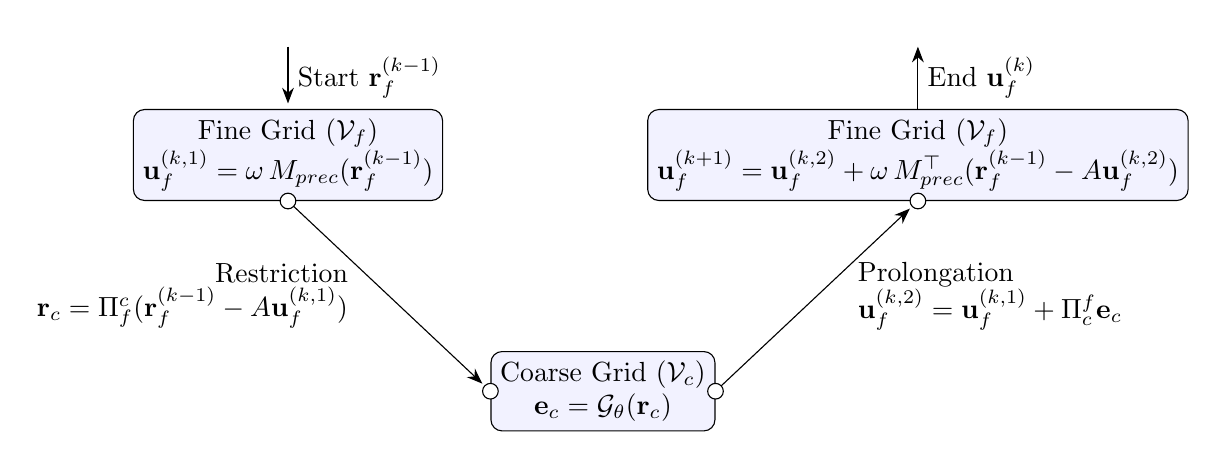
\begin{tikzpicture}[
        scale=1.0,
        transform shape,
        >={Stealth[length=2mm]},
        node distance=2.5cm,
        level/.style={draw, rectangle, rounded corners, minimum width=2.5cm, minimum height=1cm, align=center, fill=blue!5},
        op/.style={draw, circle, inner sep=2pt, fill=white},
        label_text/.style={font=\small\bfseries}
        ]

        % Nodes
        \node[level] (FinePre) at (0, 0) {Fine Grid ($\mathcal{V}_f$) \\ $\mathbf{u}_f^{(k,1)} =\omega \,  M_{prec}(\mathbf{r}_f^{(k-1)})$};
        \node[level] (Coarse) at (4, -3) {Coarse Grid ($\mathcal{V}_c$) \\ $\mathbf{e}_c = \mathcal{G}_{\theta}(\mathbf{r}_c)$};
        \node[level] (FinePost) at (8, 0) {Fine Grid ($\mathcal{V}_f$) \\ $\mathbf{u}_f^{(k+1)} = \mathbf{u}_f^{(k,2)} + \omega \,  M_{prec}^{\top} (\mathbf{r}_f^{(k-1)} - A \mathbf{u}_f^{(k,2)})$};

        % Input/Output invisible nodes
        \node (Input) at (0, 1.5) {};
        \node (Output) at (8, 1.5) {};

        % Arrows
        % Input -> Pre
        \draw[->, shorten >=2pt] (Input) -- (FinePre) node[midway, right] {Start $\mathbf{r}_f^{(k-1)}$};

        % Pre -> Coarse (Restriction)
        \draw[->, shorten >=4pt] (FinePre.south) -- (Coarse.west)
        node[midway, left, align=right, xshift=-0.4cm] {Restriction \\ $\mathbf{r}_c = \Pi_f^c (\mathbf{r}_f^{(k-1)} - A \mathbf{u}_f^{(k,1)})$};

        % Coarse -> Post (Prolongation)
        \draw[->, shorten >=4pt] (Coarse.east) -- (FinePost.south)
        node[midway, right, align=left, xshift=0.4cm] {Prolongation \\ $\mathbf{u}_f^{(k,2)} = \mathbf{u}_f^{(k,1)} + \Pi_c^f \mathbf{e}_c$};

        % Post -> Output
        \draw[->] (FinePost) -- (Output) node[midway, right] {End $\mathbf{u}_f^{(k)}$};

        % Visual cues for V-cycle shape
        % Circles at corners for emphasis
        \node[op] at (FinePre.south) {};
        \node[op] at (Coarse.west) {};
        \node[op] at (Coarse.east) {};
        \node[op] at (FinePost.south) {};

    \end{tikzpicture}
    \caption{Visual representation of one iteration of the two-level V-cycle preconditioner. The algorithm iterates between smoothing on the fine grid and correcting error modes on the coarse grid using the IgaNet.}
    \label{fig:v_cycle}
\end{figure}

To transfer both coarse grid corrections and residuals between different levels of the V-cycle preconditioner, we use the prolongation and restriction operators in Eqs. \eqref{eq:prolongation} and \eqref{eq:restriction}, respectively.
The prolongation and restriction operator adopted in this paper are based on an $L^2$ projection \cite{brenner2008mathematical, sampath2010parallel}.
\\
The prolongation operator $\Pi_{c}^f: \mathcal{V}_{c} \rightarrow \mathcal{V}_{f}$ is given by
\begin{equation}
    \label{eq:Pfc}
    \Pi_{c}^f(\mathbf{v}_{c}) = (M_f)^{-1} P_{c}^f \ \mathbf{v}_{c},
\end{equation}
where the mass matrix $M_f$ and transfer matrix $P_{c}^f$ are defined, respectively, as follows:
\begin{equation} \label{PM}
    ( M_{f})_{(i,j)} := \int_{\Omega} B_{i,f} B_{j,f}  \hspace{0.1cm} \text{d} \Omega,  \hspace{1.0cm} (P_{c}^f)_{(i,j)} :=  \int_{\Omega} B_{i,f} B_{j,c}  \hspace{0.1cm} \text{d} \Omega,
\end{equation}
where $\{B_{i,f}\}_i$ and $\{B_{j,c}\}_j$ denote the basis functions of $\mathcal{V}_f$ and $\mathcal{V}_c$ respectively.
\\
The residuals are restricted from fines to the coarse level by projection onto the space $\mathcal{V}_{c}$. The restriction operator  $\Pi_{f}^{c}: \mathcal{V}_{f} \rightarrow \mathcal{V}_{c}$ is defined by
\begin{equation}
    \label{eq:Pcf}
    \Pi_{f}^{c}(\mathbf{v}_{f}) = (M_{c})^{-1} (P_{c}^f)^\top \ \mathbf{v}_{f},
\end{equation}
where $P_{c}^f$ is defined as in \eqref{PM} and $M_{c}$ is the mass matrix of the coarse grid, explicitly
\begin{equation*}
    ( M_{c})_{(i,j)} := \int_{\Omega} B_{i,c} B_{j,c}  \hspace{0.1cm} \text{d} \Omega.
\end{equation*}
\begin{rmk}[Multilevel preconditioning]\label{rmk:multilevel_preconditioning}
    We underline that the introduction of the neural network in the coarse-grid correction is a novel approach that is beneficial for computational efficiency.
    In general, we allow the IgaNet to be defined on a coarser discretization than the problem we are solving, i.e., $h_{c} \ge h$ and $p_{c} \le p$.  Indeed, it allows to adopt the same trained IgaNet for different discretizations of the original continuous problem, significantly speeding up the construction of the preconditioner, avoiding the re-training of the IgaNet. Moreover, if the IgaNet is trained at the same discretization as isogeometric discretization of the problem ($\mathcal{V}_{f} = \mathcal{V}_{c}$), the projection and prolongation operators are simply the identity operator and our preconditioner reduces to the technique proposed in \cite{lee2025hybrid}.
\end{rmk}
\begin{rmk}[Richardson relaxation parameter]
    \label{rmk:rich_par}
    The parameter $\omega$ is an estimate of the optimal Richardson parameter $\omega_{opt}:=\frac{2}{\lambda_{\min}(A)+\lambda_{\max}(A)}$, where $\lambda_{\min}(\cdot)$ and $\lambda_{\max}(\cdot)$ are the minimum and maximum of the eigenvalues of a given matrix, respectively.
    We estimate $\lambda_{\min}(A)$ and $\lambda_{\max}(A)$ as follows. Let $J = D\mathcal{F}$ be the Jacobian of $\mathcal{F}$ and define the parametric diffusion tensor $\mathcal{G} = |\det(J)| \, (J^{\top} J)^{-1}$, which arises from the change of variables in the bilinear form. We compute
    \begin{equation*}
        \widetilde{\lambda}_{M} = \max_{\mathbf{x}}\ \lambda_{\max}(\mathcal{G}(\mathbf{x})), \qquad \widetilde{\lambda}_{m} = \min_{\mathbf{x}}\ \lambda_{\min}(\mathcal{G}(\mathbf{x})),
    \end{equation*}
    where the extrema are taken over all quadrature points $\mathbf{x}$ in the mesh, and set
    \begin{equation*}
        \omega = \frac{2}{\widetilde{\lambda}_{M} + \widetilde{\lambda}_{m}}.
    \end{equation*}
\end{rmk}


\subsubsection{Classical preconditioners as smoothers}\label{sec:classical_smoothers}
In our experiments, we employ the following classical preconditioners as smoothers $M_{prec}$:
\begin{itemize}
    \item \textbf{Jacobi:} The classical diagonal preconditioner, defined as $M_{Jac} = \text{diag}(A)^{-1}$, where $\text{diag}(A)$ denotes the diagonal of the stiffness matrix.
    \item \textbf{Gauss-Seidel:} A triangular preconditioner based on the lower triangular part of $A$, defined as $M_{GS} = (L + D)^{-1}$, where $D = \text{diag}(A)$ and $L$ is the strictly lower triangular part of $A$.
    \item \textbf{Fast Diagonalization (FD):} A tensor-product preconditioner that exploits the Kronecker structure of the IGA operators. We briefly recall its main features and we refer to \cite{sangalli2016isogeometric} for details on its use in IGA and to \cite{Lynch1964} for its first appearance. The preconditioner that we consider is defined as
          $$
              M_{FD}=\widehat{A}+\widehat{M},
          $$
          where $(\widehat{A})_{(i,j)}=\int_{\widehat{\Omega}}\nabla\widehat{B}_i\cdot\nabla\widehat{B}_j \mathrm{d}\widehat{\Omega}$ and $(\widehat{M})_{(i,j)}=\int_{\widehat{\Omega}}\widehat{B}_i\widehat{B}_j \mathrm{d}\widehat{\Omega}$  are the stiffness matrix and the mass matrix, respectively, discretized in the parametric domain and $\alpha\geq 0$. Note that, differently than \cite{sangalli2016isogeometric}, we also add a mass matrix, to ensure invertibility of $ M_{FD}$, as we deal with pure homogeneous Neumann conditions.
          We have that
          \begin{equation}
              \label{eq:FD}
              M_{FD}=\sum_{i=1}^d \widehat{M}_d\otimes\dots\otimes\widehat{M}_{i+1}\otimes\widehat{A}_i\otimes\widehat{M}_{i+1}\otimes \dots\otimes \widehat{M}_1 + \widehat{M}_d\otimes \dots \otimes \widehat{M}_1 ,
          \end{equation}
          where $\widehat{A}_i$ and $\widehat{M}_i$ are the stiffness and mass matrices built in the univariate spline spaces. Then, we compute the generalized eigendecomposition of the pencils $(\widehat{A}_i, \widehat{M}_i)$ and we get
          $$
              \widehat{A}_iU_i=\widehat{M}_iU_i\Lambda_i \ \text{ and }\ U_i^{\top}\widehat{M}_iU_i=\mathbb{I},
          $$
          where $U_i$ is the matrix of generalized eigenvector and $\Lambda_i$ is the diagonal matrix of generalized eigenvalues, while $\mathbb{I}$ denotes the identity matrix of conforming order. We then get the factorizations
          $$
              \widehat{A}_i= U_i^{-\top}\Lambda_iU_i^{-1} \ \text{ and } \ \widehat{M}_i=U_i^{-\top}U_i^{-1},
          $$
          that can be used in \eqref{eq:FD} to get
          $$
              M_{FD}= (U_d\otimes\dots \otimes U_1)^{-\top}(\mathbf{\Lambda}_s + \mathbb{I})(U_d\otimes\dots \otimes U_1)^{-1},
          $$
          where $\mathbf{\Lambda}_s:=\sum_{i=1}^d \mathbb{I}\otimes \dots \otimes \mathbb{I}\otimes \Lambda_i\otimes \mathbb{I}\otimes\dots\otimes \mathbb{I}$. Then, its inverse can be easily obtained exploiting the properties of Kronecker products as
          $$
              M_{FD}^{-1}= (U_d\otimes\dots \otimes U_1)(\mathbf{\Lambda}_s +\mathbb{I})^{-1}(U_d\otimes\dots \otimes U_1)^{\top}.
          $$
          For more details on its efficient application, we refer to \cite{sangalli2016isogeometric}.
\end{itemize}

%%%%%%%%%%%%%%%%%%%%%%%%%%%%%%%%%%%%%%%%%
%% Section
%%%%%%%%%%%%%%%%%%%%%%%%%%%%%%%%%%%%%%%%%
\section{Methodology and experiments for fixed domain}\label{sec:experiments_fixed}
In this section we present some numerical experiments to show the performance of the IgaNet architecture as preconditioner to approximate the solution operator of the Poisson problem defined in Eq. \eqref{eq:poisson_strong}. In this Section, we consider the case where the input of the neural network consists only on the right-hand side $\mathbf{f}$. The domain $\Omega$ is considered fixed and, specifically, it is a B-spline approximation of a quarter of an annulus with internal radius equal to 1 and external radius equal to 2. In particular, we want to show how the IgaNet is able to generalize over different right-hand side functions. In Sec. \ref{sec:experiments_rhs_domain} we will consider the case of variable domains, where the input of the neural network includes both the right-hand side and the control points of the domain.

%%%%%%%%%%%%%%%%%%%%%%%%%%%%%%%%%%%%%%%%%
\subsection{Multi-Layer Perceptron and Skip Connections}\label{sec:mlp_skip}
We  briefly define \textbf{Multi-Layer Perceptron (MLP)} as a class of feedforward neural networks. An MLP with \( L \) layers is defined by the following recursive relation. Let $L\in \N$, $n_l\in \N$ for $l=0, \dots, L$, then let \( \mathbf{x} \in \R^{n_0} \) be the input vector and \( \mathbf{x}^{(l)} \in \R^{n_l} \) denote the output of the \( l \)-th layer for \( l = 1, 2, \dots, L+1 \).
\[
    \begin{cases}
        \mathbf{x}^{(l)} = \sigma\left(W^{(l)} \mathbf{x}^{(l-1)} + \mathbf{b}^{(l)}\right), \quad l = 1, 2, \dots, L, \\
        \mathbf{x}^{(L+1)} = W^{(L+1)} \mathbf{x}^{(L)} + \mathbf{b}^{(L+1)},
    \end{cases}
\]
where \( \mathbf{x}^{(0)} := \mathbf{x} \) is the input to the first layer. Moreover, \( W^{(l)} \in \R^{n_l \times n_{l-1}}\), \( \mathbf{b}^{(l)} \in \R^{n_l} \) for \( l = 1, \dots, L+1 \), are the weight matrix and the bias vector of the \( l \)-th layer, respectively. The function \( \sigma: \R \to \R \) is a nonlinear activation function, that is applied element-wise. In Fig. \ref{fig:mlp} we show a schematic representation of an MLP with \( L=2 \) hidden layers.

\begin{figure}[!ht]
    \centering
    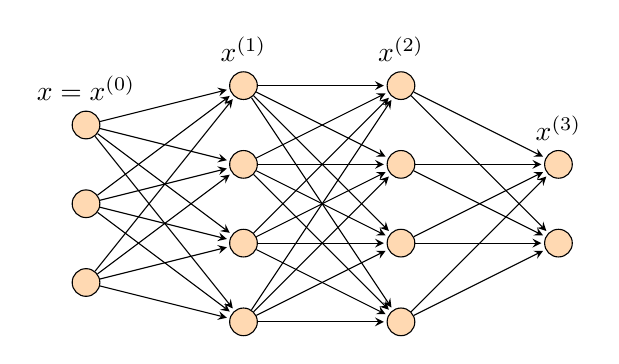
\begin{tikzpicture}[
            >=stealth,
            shorten >=1pt,
            auto,
            node distance=2cm,
            neuron/.style={draw, circle, fill=orange!30, minimum size=10pt, inner sep=0pt},
            layer/.style={thick, draw=black!50, rectangle, fill=black!10, minimum height=4em},
        ]

        % Draw the input layer nodes
        \foreach \name / \y in {1}
        \node[neuron, label=above:{$x = x^{(0)}$}] (I-\name) at (0,-\y-0.5) {};
        \foreach \name / \y in {2,...,3}
        \node[neuron] (I-\name) at (0,-\y-0.5) {};

        % Draw the hidden layer nodes
        \foreach \name / \y in {1}
        \node[neuron, label=above:{$x^{(1)}$}] (H1-\name) at (2.0,-\y) {};
        \foreach \name / \y in {2,...,4}
        \node[neuron] (H1-\name) at (2.0,-\y) {};

        \foreach \name / \y in {1}
        \node[neuron, label=above:{$x^{(2)}$}] (H2-\name) at (4.0,-\y) {};
        \foreach \name / \y in {2,...,4}
        \node[neuron] (H2-\name) at (4.0,-\y) {};

        % Draw the output layer node
        \foreach \name / \y in {2}
        \node[neuron, label=above:{$x^{(3)}$}] (O-\name) at (6.0,-\y) {};
        \foreach \name / \y in {3}
        \node[neuron] (O-\name) at (6.0,-\y) {};

        % Connect every node in the input layer with every node in the
        % hidden layer.
        \foreach \source in {1,...,3}
        \foreach \dest in {1,...,4}
        \draw[-stealth] (I-\source) -- (H1-\dest);

        \foreach \source in {1,...,4}
        \foreach \dest in {1,...,4}
        \draw[-stealth] (H1-\source) -- (H2-\dest);

        % Connect every node in the hidden layer with the output layer
        \foreach \source in {1,...,4}
        \foreach \dest in {2,3}
        \draw[-stealth] (H2-\source) -- (O-\dest);
    \end{tikzpicture}%
    \caption{Schematic representation of a MLP with $L=2$ hidden layers. Circles represent neurons, which correspond to the scalar components of the layer vectors $\mathbf{x}^{(l)}$. Arrows denote the weighted connections between layers, representing the affine transformations (multiplication by weights $W^{(l)}$ and addition of bias $\mathbf{b}^{(l)}$) followed by the non-linear activation $\sigma$.}
    \label{fig:mlp}
\end{figure}
An important concept in neural network architecture are the \textbf{skip connections/residual blocks}, which allow the direct passage of information from earlier layers to later layers, bypassing one or more intermediate layers. This technique was introduced to address the vanishing gradient problem, which hinders the training of deep networks \cite{he2016deep}. In particular, a residual block computes its output by adding the input of the block to its own output. Formally, let \( \mathbf{x} \in \R^{n}, \ n \in \N \) be the input to a residual block, and let \( \mathcal{C}:\R^n \to \R^{n} \) represent the series of operations within the block. In the context of MLPs described above, the function $\mathcal{C}$ corresponds to a sequence of one or more hidden layers. The final output \( \mathbf{y} \in \R^{n} \) of the residual block is then
\begin{equation}
    \mathbf{y} = \mathbf{x} + \mathcal{C}(\mathbf{x}).
    \label{eq:skip_connection}
\end{equation}
The identity mapping \( \mathbf{x} \) is the skip connection. This formulation allows the network to learn residual functions, or adjustments to the identity, rather than learning the entire transformation. This has been shown to significantly ease the training of deep networks and improve their performance \cite{he2016identity}. We give a schematic representation of an MLP with $L=5$ hidden layers and two residual blocks in Fig. \ref{fig:mlp_deep}.
\begin{ass}
    In all the numerical experiments presented in this work, we assume that all hidden layers of the MLP share the same width, i.e. $n_l = n_{neuron}$ for all $l = 1, \dots, L$. Consequently, the weight matrices for the intermediate layers are square matrices in $\R^{n_{neuron} \times n_{neuron}}$. Moreover, the input and output dimensions are the same, i.e., $n_0=n_{L+1}=\text{dim}(\mathcal{V}_h)$.
\end{ass}

\begin{figure}[!ht]
    \centering
    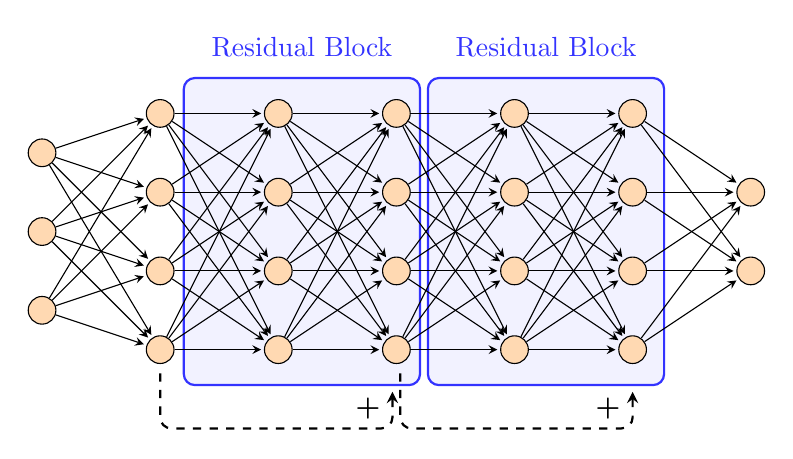
\begin{tikzpicture}[
            >=stealth,
            shorten >=1pt,
            auto,
            node distance=1.5cm,
            neuron/.style={draw, circle, fill=orange!30, minimum size=10pt, inner sep=0pt},
            layer/.style={thick, draw=black!50, rectangle, fill=black!10, minimum height=4em},
            skip/.style={->, thick, dashed, rounded corners}
        ]

        % ======================================
        % Bounding box for Residual Block
        % ======================================
        \draw[blue!80, thick, rounded corners, fill=blue!5] (1.8, -0.55) rectangle (4.8, -4.45);
        \node[blue!80] at (3.3, -0.15) {Residual Block};

        \draw[blue!80, thick, rounded corners, fill=blue!5] (4.9, -0.55) rectangle (7.9, -4.45);
        \node[blue!80] at (6.4, -0.15) {Residual Block};

        % ======================================
        % Neurons
        % ======================================
        % L1: Input (x) at x=0.0
        \foreach \name / \y in {1,2,3}
        \node[neuron] (L1-\name) at (0.0,-\y-0.5) {};
        % \node[above] at (0.0,-1.0) {$\mathbf{h}^{(0)}$};

        % L2: Hidden at x=1.5
        \foreach \name / \y in {1,...,4}
        \node[neuron] (L2-\name) at (1.5,-\y) {};
        % \node[above] at (1.5,-0.5) {L2};

        % L3: Hidden at x=3.0
        \foreach \name / \y in {1,...,4}
        \node[neuron] (L3-\name) at (3.0,-\y) {};
        % \node[above] at (3.0,-0.5) {L3};

        % L4: Hidden at x=4.5
        \foreach \name / \y in {1,...,4}
        \node[neuron] (L4-\name) at (4.5,-\y) {};
        % \node[above] at (4.5,-0.5) {L4};

        % L5: Hidden at x=6.0
        \foreach \name / \y in {1,...,4}
        \node[neuron] (L5-\name) at (6.0,-\y) {};
        % \node[above] at (6.0,-0.5) {L5};

        % L6: Hidden at x=7.5
        \foreach \name / \y in {1,...,4}
        \node[neuron] (L6-\name) at (7.5,-\y) {};
        % \node[above] at (7.5,-0.5) {L6};

        % L7: Hidden (Removed)
        % \foreach \name / \y in {1,...,4}
        % \node[neuron] (L7-\name) at (9.0,-\y) {};
        % \node[above] at (9.0,-0.5) {L7};

        % L8: Output (y) at x=9.0 (Shifted back)
        \foreach \name / \y in {2,3}
        \node[neuron] (L8-\name) at (9.0,-\y) {};
        % \node[above] at (10.5,-1.5) {$y$ (L8)};


        % ======================================
        % Sequential Connections
        % ======================================
        % L1 -> L2
        \foreach \source in {1,2,3}
        \foreach \dest in {1,...,4}
        \draw[-stealth] (L1-\source) -- (L2-\dest);

        % L2 -> L3
        \foreach \source in {1,...,4}
        \foreach \dest in {1,...,4}
        \draw[-stealth] (L2-\source) -- (L3-\dest);

        % L3 -> L4
        \foreach \source in {1,...,4}
        \foreach \dest in {1,...,4}
        \draw[-stealth] (L3-\source) -- (L4-\dest);

        % L4 -> L5
        \foreach \source in {1,...,4}
        \foreach \dest in {1,...,4}
        \draw[-stealth] (L4-\source) -- (L5-\dest);

        % L5 -> L6
        \foreach \source in {1,...,4}
        \foreach \dest in {1,...,4}
        \draw[-stealth] (L5-\source) -- (L6-\dest);

        % L6 -> L8 (changed from L6->L7->L8)
        \foreach \source in {1,...,4}
        \foreach \dest in {2,3}
        \draw[-stealth] (L6-\source) -- (L8-\dest);


        % ======================================
        % Skip Connections
        % ======================================
        % Skip 1: From L2 to L4
        % Path: L2 (x=1.5) -> down -> across -> L4 (x=4.5)
        \draw[skip] (1.5, -4.3) -- (1.5, -5) -- (4.45, -5) -- (4.45, -4.5)
        node[midway, inner sep=4pt, font=\bfseries] {+};

        % Skip 2: From L4 to L6
        % Path: L4 (x=4.5) -> down -> across -> L6 (x=7.5)
        \draw[skip] (4.55, -4.3) -- (4.55, -5) -- (7.5, -5) -- (7.5, -4.5)
        node[midway, inner sep=4pt, font=\bfseries] {+};


    \end{tikzpicture}%
    \caption{Architecture of a MLP with two sequential residual blocks. The skip connections (dashed lines) allow the network to learn residual functions by adding the input of each block directly to its output. The highlighted blue regions indicated the two residual blocks.}
    \label{fig:mlp_deep}
\end{figure}

%%%%%%%%%%%%%%%%%%%%%%%%%%%%%%%%%%%%%%%%%
\subsection{Dataset generation and IgaNet training}\label{sec:experiments_rhs}
\begin{ass}
    In the remainder of this work, we will focus exclusively on two-dimensional problems, i.e., problems defined on a domain $\Omega \subset \R^d$ with $d=2$.
\end{ass}
\subsubsection{Dataset generation}\label{sec:dataset_generation}
%As first experiment we want to see how the IgaNet behaves when we vary the right-hand side of the problem on a two-dimensional fixed domain. 
We generate the data on the reference domain $\widehat{\Omega}$ as functions $\hat{f}$, which are then mapped to the physical domain $\Omega = \mathcal{F}(\widehat{\Omega})$ via the composition with the inverse of the geometric parametrization, i.e., $f = \hat{f} \circ \mathcal{F}^{-1}$. The parametric source terms $\hat{f}$ are sampled using Gaussian random fields (GRFs) \cite{adler2010geometry} with an exponential covariance function, i.e.
\begin{equation}
    Cov(\hat{f}(\mathbf{x}), \hat{f}(\mathbf{y})) = \sigma^2 exp\left(-\frac{\|\mathbf{x} - \mathbf{y}\|}{\lambda}\right),
    \label{eq:covariance}
\end{equation}
with correlation length $\lambda = 2d^2$, $d = 0.05$ and standard deviation $\sigma = 1$, according to what is done in \cite{kopanivcakova2025deeponet}.
The dataset is then normalized in order to satisfy the condition $\sum_{i=1}^{n} \mathbf{f}_i=0$ (based on Sec. \ref{sec:model_problem}). For each sample of the source term, we compute the corresponding high-fidelity solution using the GeoPDEs library \cite{de2011geopdes} and Matlab backslash “ \textbackslash”  to solve the linear systems. In total, we generate $N_{data} = 20^{\cdot}000$ input-output pairs $\{(\mathbf{f}^{(i)}, \mathbf{u}^{(i)})\}_{i=1}^{N_{data}}$, where $\mathbf{f}^{(i)}$ is the vector of the discretized source term and $\mathbf{u}^{(i)}$ is the vector of the discretized high-fidelity solution.
The dataset is split into training set (80\% of the data), validation set (10\% of the data) and test set (10\% of the data). The training set is used to train the IgaNet, the validation set is used to tune the hyperparameters of the IgaNet and the test set is used to evaluate the performance of the IgaNet.

\subsubsection{Loss function}
To measure the error done by the IgaNet model, we compute the mean $\ell^2$ error between the approximated solution $\mathcal{G}_\theta(\mathbf{f})\in \R^n$ and the target solution $\mathbf{u}\in \R^n$, i.e.
\begin{equation}
    Loss\left(\mathbf{u},\, \mathcal{G}_\theta(\mathbf{f})\right)
    %= \frac{1}{n}\|\mathbf{u} - \mathcal{G}_\theta(\mathbf{f})\|_{\ell^2}
    = \left(\frac{1}{n}\sum_{i=1}^{n} |\mathbf{u}_i - \mathcal{G}_\theta(\mathbf{f})_i|^2\right)^{1/2},
    \label{eq:l2_error}
\end{equation}
where $n$ is the number of degrees of freedom. The training process of the IgaNet model consists in approximating the parameters of the model that satisfies the following minimization problem over all the training set $\{(\mathbf{f}^{(i)}, \mathbf{u}^{(i)})\}_{i=1}^{n_{data}}$
\[
    \underset{\theta\in\Theta}{argmin} \ \ \frac{1}{n_{data}} \sum_{i=1}^{n_{data}} Loss\left(\mathbf{u}^{(i)},\, \mathcal{G}_\theta(\mathbf{f}^{(i)})\right).
\]
where $n_{data}$ is the number of data in the training set and $\Theta$ is the set containings all the trainable IgaNet's parameters.
In all our experiments, the IgaNet is trained using AdamW optimizer \cite{loshchilov2019decoupledweightdecayregularization}.

\subsubsection{Hyperparameters optimization}\label{sec:hyperparameters_optimization}
The efficacy of the IgaNet architecture in approximating the solution operator is intrinsically linked to the optimal selection of its hyperparameters. Given the non-trivial influence of network depth, width, and training dynamics on convergence and generalization, we conduct a systematic hyperparameter optimization process. This approach allows us to explore a comprehensive search space and identify the configuration that minimizes the validation error while ensuring computational efficiency. Specifically, we fix the AdamW optimizer for $5000$ epochs and with a batch size of $100$, then we target the optimization of the following hyperparameters:
\begin{itemize}
    \item \textbf{Learning rate} ($\lambda \in [10^{-4}, 10^{-2}]$): Controls the step size during gradient descent optimization.

    \item \textbf{Learning rate reduction factor} ($\eta \in [0.75, 0.99]$): The multiplicative factor used in the step learning rate scheduler. This scheduler decays the learning rate by $\eta$ every fixed number of epochs (set to 250 in our experiments) to progressively refine the optimization steps as training advances.

    \item \textbf{Regularization factor} ($w \in [10^{-6}, 10^{-3}]$): The weight decay coefficient applied within the AdamW optimizer. This parameter prevents overfitting by penalizing large weights.

    \item \textbf{Dropout rate} ($\gamma \in [0.00, 0.50]$): Probability of randomly dropping neurons during training to improve generalization and reduce overfitting, for more details see \cite{srivastava2014dropout}.

    \item \textbf{Number of residual blocks} ($1 \le L \le 8$): Total number of residual blocks in the network architecture, see Sec. \ref{sec:mlp_skip}.

    \item \textbf{Number of neurons per residual block} ($n_{\text{neuron}} \in \{100k \mid k = 1, \ldots, 10\}$): Width of each residual block, that is the dimension of the vectors in Eq. \eqref{eq:skip_connection}. For semplicity, we take the same number of neurons for all the residual blocks.

    \item \textbf{Number of layers per block} ($L_{\text{block}} \in [0, 8]$): Depth of each residual block, controlling the number of transformation layers within each block.

    \item \textbf{Activation function} ($\sigma \in \{\text{GELU}, \text{LReLU}, \text{ReLU}, \tanh\}$): We test four different activation functions, i.e., Gaussian Error Linear Units function (GELU, \cite{hendrycks2016gaussian}), Leaky Rectified Linear Units function (LReLU), Rectified Linear Units function (ReLU) and Hyperbolic tangent function ($\tanh$).
\end{itemize}
We evaluate $200$ distinct hyperparameter configurations, sampled from the search space defined above, to identify the optimal IgaNet's architecture. This search is performed using the HyperNOs library \cite{ghiotto2025hypernos}, which relies on the Tree-structured Parzen Estimators algorithm \cite{watanabe2023tree, bergstra2015hyperopt} for the hyperparameter configuration selection, and on the ASHA scheduler \cite{li2020massivelyparallelhyperparametertuning} to automatically prune unpromising trials. This adaptive approach provides a significant advantage over exhaustive grid search, as it concentrates computational resources on the most promising regions of the hyperparameter space and avoids wasting time on poor-performing configurations. The time needed for each hyperparameter optimization test strongly depends on the dimension of the datasets and the configuration of the search space. Our tests take up to one day each on a single $4090$ NVIDIA GPU.

\subsubsection{IgaNet training}
%We consider the homogeneous Poisson problem, see Eq. \eqref{eq:poisson_strong}, where the computational domain $\Omega$ is a  quarter of annulus with internal radius equal to 1 and external radius equal to 2. 
We examine different discretizations for the problem \eqref{eq:discrete_problem}, by employing B-spline spaces with a fixed degree $p=3$ and varying levels of domain refinement.
In particular, we set the number of subdivisions in each parametric direction to $2^\reflevel$, with $\reflevel \in \{3, 4, 5\}$. For each discretization, we generate the corresponding dataset (see Sec. \ref{sec:dataset_generation}) and perform hyperparameter optimization for the IgaNet (see Sec. \ref{sec:hyperparameters_optimization}).

The optimal hyperparameters identified through this process are summarized in Table \ref{table:fixed_rhs_ray_hyperparams_A}. Subsequently, for each discretization level, we train the IgaNet model three times with different random weight initializations. The corresponding results, including mean and standard deviation of both training loss and test error, are presented in Table \ref{table:fixed_rhs_results_A}. These findings demonstrate that the IgaNet architecture effectively approximates the solution operator with high accuracy and low variance across different initializations, thereby validating its suitability as a preconditioner.
We can also observe that increasing the refinement level $\reflevel$ leads to a higher number of degrees of freedom in Eq. \eqref{eq:discrete_problem}, which increases the dimensionality of both the input and output spaces. This added complexity makes the learning task more challenging, resulting in a slight increase in the approximation error as $\reflevel$ grows.

\begin{table}[!ht]
    \centering
    \begin{tabular}{cccccccccc}
        \toprule
         & discretization & $\lambda$ & $\eta$ & $w$                & $\gamma$ & $L$ & $n_{neuron}$ & $L_{block}$ & $\sigma$ \\
        \cmidrule{1-10}
         & $\reflevel=3$  & $0.0007$  & $0.75$ & $4.3\cdot 10^{-4}$ & $0.19$   & $3$ & $500$        & 3           & GELU     \\
         & $\reflevel=4$  & $0.0002$  & $0.77$ & $0.9\cdot 10^{-4}$ & $0.20$   & $4$ & $700$        & 3           & GELU     \\
         & $\reflevel=5$  & $0.0001$  & $0.98$ & $1.0\cdot 10^{-4}$ & $0.16$   & $2$ & $1000$       & 2           & ReLU     \\
        \bottomrule
    \end{tabular}
    \caption{Optimal hyperparameters for the IgaNet architecture found with the optimization process for varying problem discretizations.}
    \label{table:fixed_rhs_ray_hyperparams_A}
\end{table}
\begin{table}[!ht]
    \centering
    \begin{tabular}{ccccc}
        \toprule
        discretization & training loss                    & test error                       & n. of params. & train. time (min.) \\
        \cmidrule{1-5}
        $\reflevel=3$  & $(4.51 \pm 0.04)\cdot 10^{-8}$   & $(4.68 \pm 0.04)\cdot 10^{-8}$   & $1.6$M        & 45                   \\
        $\reflevel=4$  & $(5.50 \pm 0.12)\cdot 10^{-7}$   & $(6.61 \pm 0.21)\cdot 10^{-7}$   & $4.4$M        & 125                  \\
        $\reflevel=5$  & $(2.447 \pm 0.001)\cdot 10^{-5}$ & $(3.847 \pm 0.001)\cdot 10^{-5}$ & $4.5$M        & 100                  \\
        \bottomrule
    \end{tabular}
    \caption{Training results of the IgaNet architecture with optimized hyperparameters for different discretizations. Mean and standard deviation are computed over three independent runs with different random weight initializations.}
    \label{table:fixed_rhs_results_A}
\end{table}

\subsection{IgaNet as preconditioner}
In this section, we evaluate the performance of the trained IgaNet when employed as a preconditioner for the high-fidelity IGA discretization of the problem \eqref{eq:discrete_problem}.
\subsubsection{Same discretization experiments}
In this numerical experiments, we maintain an identical discretization for both the high-fidelity solver and the IgaNet (see Remark \ref{rmk:multilevel_preconditioning}), employing B-splines of degree $p=3$ and varying the number of subdivisions $2^\reflevel$ with $\reflevel \in \{3, 4, 5\}$.
The test cases are generated by sampling the right-hand side function in the parametric domain  $\hat{f}$ from a Gaussian random field with the same exponential covariance function defined in Eq. \eqref{eq:covariance} and with the same correlation length $\lambda$ used during training, but with a standard deviation $\sigma = 10$, which differs from the training value of $\sigma = 1$. This choice ensures that the preconditioner is evaluated on out-of-distribution data with respect to the magnitude of the forcing term. Then, as in the dataset generation, the right-hand side in the physical domain is obtained by composition of the inverse of the geometrical mapping, i.e. $f=\hat{f}\circ\mathcal{F}^{-1}$. An illustration of one possible right-hand side and the corresponding solution are presented in Fig. \ref{fig:input-output}. For all the plots in this section, the reported number of iterations corresponds to the average over $10$ independent runs with different realizations of $f$.
\begin{figure}[!ht]
    \centering
    \hfill
    \begin{subfigure}[b]{0.35\textwidth}
        \centering
        \includegraphics[width=\textwidth, height=0.2\textheight, keepaspectratio=false]{figures/ring-input.png}
        \caption{Right-hand side function $f$.}
        \label{fig:ring-input}
    \end{subfigure}
    \hfill
    \begin{subfigure}[b]{0.35\textwidth}
        \centering
        \includegraphics[width=\textwidth, height=0.2\textheight, keepaspectratio=false]{figures/ring-output.png}
        \caption{High-fidelity solution $u$.}
        \label{fig:ring-output}
    \end{subfigure}
    \hfill\mbox{}
    \caption{Representative training sample for the IgaNet: Fig. \ref{fig:ring-input} displays a realization of the right-hand side function $f$, generated from a Gaussian Random Field with exponential covariance; Fig. \ref{fig:ring-output} shows the corresponding high-fidelity solution $u$ to the Poisson problem \eqref{eq:poisson_strong} on the quarter-annulus domain.}
    \label{fig:input-output}
\end{figure}
We compare the convergence properties of classical preconditioners, namely Jacobi, Gauss-Seidel, and Fast Diagonalization, against their enhanced counterparts where the IgaNet is applied as a coarse-grid correction. Moreover, for all the preconditioners we adopt the V-cycle approach presented in Sec. \ref{sec:preconditioning_strategy}.
Finally, for the F-GMRES solver (see Remark \ref{rmk:fgmres}), we utilize a relative stopping tolerance of $10^{-8}$.
\\
The convergence results are reported in Fig. \ref{fig:neumann_iganet_rhs_comparison}, which demonstrates that the IgaNet significantly reduces the iteration count required for convergence across all classical preconditioners. Specifically, we observe an improvement factor of approximately $3$ for both Jacobi and Gauss-Seidel methods. For the Fast Diagonalization method, we achieve a reduction factor of $3$ for $\reflevel \in \{3, 4\}$ and a factor of $2$ for $\reflevel=5$. Furthermore, it is worth noting that the FD method combined with the IgaNet preconditioner conserves one of the most important features of FD, indeed, the number of iterations remains nearly constant as the refinement level $\reflevel$ increases.

\begin{rmk}[Flexible GMRES]\label{rmk:fgmres}
   We address the solution of the linear system \eqref{eq:discrete_problem} using an iterative method. Since the IgaNet is based on a non-linear neural network architecture, it effectively defines a variable preconditioner. Consequently, standard Krylov subspace methods are not applicable; instead, we adopt the Flexible GMRES (F-GMRES, \cite{saad1993flexible}) algorithm, which specifically allows for variable preconditioning at each iteration.
\end{rmk}

\begin{figure}[!ht]
    \centering
    \includegraphics[width=\textwidth]{figures/neumann_iganet_rhs_comparison.png}
    \caption{Convergence comparison between the classical preconditioners (Jacobi, Gauss-Seidel and Fast Diagonalization) and the same preconditioners combined with the IgaNet, for different discretization of the problem. In the left and central figure we report the number of iterations needed to reach convergence for every preconditioner choice and for every level of discretization, while in the right figure we report the factor of gain with respect to the non-preconditioned F-GMRES (dashed line). All reported iteration counts correspond to averages over $10$ independent runs with different right-hand sides sampled from a Gaussian random field with the same correlation length as in training but with $\sigma=10$.}
    \label{fig:neumann_iganet_rhs_comparison}
\end{figure}

\subsubsection{Different discretization experiments}
In this subsection, we investigate the robustness of the IgaNet preconditioner with respect to the discretization parameters. While the previous results were obtained by matching the discretization level of the IgaNet with that of the high-fidelity solver, we now investigate the generalization capabilities of our preconditioner across different discretization levels. Specifically, we fix the IgaNet trained with degree $p=3$ and refinement level $\reflevel=3$, and evaluate its performance in the multilevel preconditioner for problems discretized with degrees $p \in \{3, 4\}$ and varying refinement levels $\reflevel \in \{3, 4, 5, 6\}$.
The results are reported in Fig. \ref{fig:neumann_iganet_multilevel}. By comparing Fig. \ref{fig:neumann_iganet_multilevel_p3} with Fig. \ref{fig:neumann_iganet_rhs_comparison}, we can directly assess the generalization capabilities with respect to the  refinement level $\reflevel$. For $\reflevel=3$, where the IgaNet matches the problem discretization, indeed the results are identical. For finer discretizations ($\reflevel=4, 5, 6$), although there is a slight decrease in performance compared to the matched case, the preconditioner still yields a reduction in iteration count by a factor of $2$-$3$ compared to the non-preconditioned solver. This highlights the efficiency gain of avoiding re-training.
In Fig. \ref{fig:neumann_iganet_multilevel_p4}, we observe the performance when the preconditioner acts across both different degrees and refinement levels. Indeed, the IgaNet is trained with $p=3$ but applied to a problem with $p=4$. We observe a degradation in the performance of Jacobi and Gauss-Seidel smoothers, with improvement factors dropping to between $1$ and $2$. Conversely, the Fast Diagonalization method combined with IgaNet retains its robust properties, exhibiting an iteration count that remains nearly constant with respect to both $\reflevel$ and $p$.
\\
This approach offers significant computational advantages, as it enables the generation of a single dataset and the training of a unique IgaNet model, which can subsequently be employed to precondition problems with varying discretizations without any additional training cost.

\begin{figure}[!ht]
    \centering
    \begin{subfigure}[b]{\textwidth}
        \centering
        \includegraphics[width=\textwidth]{figures/neumann_iganet_rhs_comparison_proj_p3.png}
        \caption{IgaNet trained with $p=3$ and $\reflevel=3$ and used as preconditioner on a problem with $p=3$ and varying $\reflevel$.}
        \label{fig:neumann_iganet_multilevel_p3}
    \end{subfigure}
    \par\bigskip
    \begin{subfigure}[b]{\textwidth}
        \centering
        \includegraphics[width=\textwidth]{figures/neumann_iganet_rhs_comparison_proj_p4.png}
        \caption{IgaNet trained with $p=3$ and $\reflevel=3$ and applied as preconditioner on a problem with $p=4$ and varying $\reflevel$.}
        \label{fig:neumann_iganet_multilevel_p4}
    \end{subfigure}
    \caption{Convergence comparison between classical preconditioners and their IgaNet-enhanced versions, using a fixed IgaNet model (trained with $p=3, \reflevel=3$) applied to varying problem discretizations. In Fig. \ref{fig:neumann_iganet_multilevel_p3} we consider problems with $p=3$ and varying $\reflevel$, assessing generalization across refinement levels. In Fig. \ref{fig:neumann_iganet_multilevel_p4} we consider problems with $p=4$ and varying $\reflevel$, assessing generalization across both refinement levels and polynomial degrees. As in Fig. \ref{fig:neumann_iganet_rhs_comparison}, the left and central plots report the iterations to convergence, while the right plots show the speedup factor with respect to the non-preconditioned F-GMRES. All reported iteration counts correspond to averages over $10$ independent runs with different right-hand sides sampled from a Gaussian random field with the same correlation length as in training but with $\sigma=10$.}
    \label{fig:neumann_iganet_multilevel}
\end{figure}

\begin{rmk}[Full multigrid preconditioner]
    In our proposed multilevel preconditioning framework, we project the residual directly from the fine discretization level, where the classical smoother is applied, to the coarse level where the IgaNet is defined. Alternatively, one could adopt a classical full multigrid approach that iteratively traverses all intermediate discretization levels. We experimentally evaluated this full multigrid strategy and observed a slight reduction in the number of iterations compared to our direct two-level approach. However, this marginal improvement in convergence rate was accompanied by a significantly higher computational cost. Consequently, we did not adopt the full multigrid scheme in this work, as the increased computational expense was not justified by the limited performance gains.
\end{rmk}

% \subsubsection{Robustness with respect to out-of-distribution source terms}
% The results presented so far were obtained using source terms sampled from a Gaussian Random Field with fixed parameters, specifically a correlation length of $d=0.05$ (and $\lambda = 2d^2$) and a standard deviation of $\sigma=1.0$, distribution that matches the training set. In this section, we investigate the robustness of the IgaNet preconditioner when applied to source terms generated from distributions that differ significantly from the training one. This analysis is crucial to assess the generalization capabilities of the model to unseen functional inputs.

% We conduct two sets of experiments on the quarter annulus geometry with the reference discretization ($p=3, \reflevel=3$):
% \begin{enumerate}
%     \item \textbf{Varying correlation length $d$:} We fix $\sigma=1.0$ and vary $d \in \{0.01, 0.05, 0.1, 0.5, 5.0\}$. The parameter $d$ controls the spatial frequency of the source term ($\lambda = 2d^2$); smaller values correspond to higher-frequency, more oscillatory functions, while larger values yield smoother functions.
%     \item \textbf{Varying standard deviation $\sigma$:} We fix $d=0.05$ and vary $\sigma \in \{0.1, 0.5, 1.0, 10.0\}$. This parameter controls the magnitude of the forcing term.
% \end{enumerate}

% The results of these out-of-distribution analyses are illustrated in Fig. \ref{fig:fixed_robustness}. As shown in both subfigures, the iteration count remains practically constant across the entire range of tested parameters. Specifically, Fig. \ref{fig:fixed_robustness_d} demonstrates that the performance is stable even for small correlation lengths, indicating robustness to high-frequency variations. Similarly, Fig. \ref{fig:fixed_robustness_sigma} confirms that the IgaNet exhibits strong generalization with respect to the magnitude of the forcing term, with the number of iterations remaining constant across varying $\sigma$. These findings suggest that the IgaNet preconditioner is not only effective within the training distribution but also maintains its performance when applied to significantly different source term distributions, highlighting its robustness and potential applicability in a wide range of scenarios.
% \begin{figure}[!ht]
%     \centering
%     \begin{subfigure}[b]{0.48\textwidth}
%         \centering
%         \includegraphics[width=\textwidth]{figures/OOD_d.png}
%         \caption{Robustness w.r.t. correlation length $d$ (with fixed $\sigma=1$).}
%         \label{fig:fixed_robustness_d}
%     \end{subfigure}
%     \hfill
%     \begin{subfigure}[b]{0.48\textwidth}
%         \centering
%         \includegraphics[width=\textwidth]{figures/OOD_sigma.png}
%         \caption{Robustness w.r.t. standard deviation $\sigma$ (with fixed $d=0.05$).}
%         \label{fig:fixed_robustness_sigma}
%     \end{subfigure}
%     \caption{Number of iterations to convergence for the F-GMRES solver preconditioned with IgaNet (trained with $p=3, \reflevel=3$) on the quarter annulus geometry, as a function of the GRF parameters $d$ and $\sigma$. The dashed line indicates the training regime parameters.}
%     \label{fig:fixed_robustness}
% \end{figure}

%%%%%%%%%%%%%%%%%%%%%%%%%%%%%%%%%%%%%%%%%
%% Section
%%%%%%%%%%%%%%%%%%%%%%%%%%%%%%%%%%%%%%%%%
\section{Methodology and experiments with varying domain}\label{sec:experiments_rhs_domain}
In this section, we extend the applicability of the IgaNet preconditioner to problems defined on several physical domains.
While the previous section focused on a fixed geometry and give the foundation of the IgaNet architecture as preconditioner, here we aim to learn a single solution operator that generalizes across different domains $\Omega$ without the need for retraining.
We will test this approach on the Poisson problem \eqref{eq:poisson_strong} defined in several geometries and with different right-hand sides. To achieve this task, we introduce the control points of the domain geometry (parametrized via splines) as a direct input to the neural network. An intuitive approach to handle both inputs (the geometry and the right-hand side) would be to simply concatenate the control points of the geometry, appropriately reshaped,  and the right-hand side into a single input vector for a standard MLP. However, this strategy presents two major drawbacks. First, mixing two mathematically distinct quantities, geometric parameters and forcing terms, makes it difficult for the network to extract meaningful features, as their statistical distributions and physical roles are fundamentally different.
Second, and more importantly, this approach fails to preserve the underlying physical structure of the problem. Specifically, the dependence of the solution on the forcing term $(\mathbf{f})$ may be linear (as in the Poisson problem) or non-linear, while the dependence on the domain geometry  is typically non-linear. A standard MLP, which processes the concatenated inputs through a sequence of non-linear layers, does not inherently preserve any potential linear structure. By separating the geometric input from the forcing term, we can design an architecture that is flexible enough to explicitly enforce linearity with respect to $\mathbf{f}$ when physically required. To address these challenges, in Sec. \ref{sec:transformer_iganet} we propose a Transformer-based architecture \cite{vaswani2017attention} tailored to the mathematical structure of the problem.

%%%%%%%%%%%%%%%%%%%%%%%%%%%%%%%%%%%%%%%%%
\subsection{Transformer based IgaNet}\label{sec:transformer_iganet}
In this section we propose a Transformer-based architecture for our IgaNet. In particular, instead of approximating the solution directly as a black-box function, we design the network to respect the linearity of the solution map with respect to the forcing term $\mathbf{f}\in \R^n$, while capturing the complex non-linear dependence on the geometry.
\\
The geometry map $\mathcal{F}$  is defined through a set of $P\in \N$  control points, that, reshaped into a matrix, we denote as $G\in \mathbb{R}^{P \times 4}$.
The dimension $4$ is due to the standard representation of NURBS with the coordinates of the control points in $\R^3$ and the weight, that is equal to $1$ for the splines geometry. % but can be extended to general NURBS geometry. 
The forcing term $\mathbf{f}\in \R^n$ is parametrized as in Sec. \ref{sec:experiments_fixed}.

The Transformer-based IgaNet is defined as
\begin{equation*}
    \mathcal{G}_{\theta}(G, \mathbf{f}) = \mathcal{A}(G, \theta) \, \mathbf{f},
\end{equation*}
where $\mathcal{A}(G; \theta)\in \R^{n\times n}$ is a matrix computed by the IgaNet and parametrized by the learnable parameters $\theta$. We will call the output of the IgaNet $\mathbf{u}_{\theta} := \mathcal{G}_{\theta}(G, \mathbf{f})$, $\mathbf{u}_{\theta}\in \R^n$.
In this formulation, the IgaNet (parametrized by $\theta$) processes only the geometric input $G$ to output the matrix $\mathcal{A}(G; \theta)$, and then multiplies it with the forcing term $\mathbf{f}$, ensuring by construction that the mapping $\mathbf{f} \mapsto \mathbf{u}_\theta$ remains linear. A detailed breakdown of the architecture follows below, for a visual representation see Fig. \ref{fig:iganet_architecture}.

\begin{itemize}
    \item \textbf{Embedding and Positional Encoding.}\\
          The geometry input is projected into a latent space and augmented with positional encoding information. Specifically, let $\mathbf{g}_i \in \R^4$ denote the $i$-th row of the input geometry $G \in \R^{P \times 4}$, representing the coordinates and weight of the $i$-th control point. We first apply a learnable affine transformation to each control point to map it into a latent feature space of dimension $\Dlat$:
          \begin{equation*}
              \widetilde{\mathbf{h}}_i = W_{in} \mathbf{g}_i + \mathbf{b}_{in}, \qquad i=1,\ldots,P,
          \end{equation*}
          where $W_{in} \in \R^{\Dlat \times 4}$ is the weight matrix and $\mathbf{b}_{in} \in \R^\Dlat$ is the bias vector. Collecting these vectors into a matrix $\tilde{H}_0 \in \R^{P \times \Dlat}$, we then inject order information via a standard sinusoidal Positional Encoding (PE):
          \begin{equation*}
              H_0 = \widetilde{H}_0 + \text{PE}(P), \qquad H_0 \in \R^{P \times \Dlat}.
          \end{equation*}
          This composite embedding strategy serves a dual purpose: the learnable affine transformation encodes the intrinsic geometric attributes (physical coordinates and weights) of each individual control point, while the positional encoding injects the crucial topological information regarding their sequential ordering within the spline control net. The positional encoding is defined as:
          \begin{equation*}
              \begin{aligned}
                  PE_{(pos, 2j)}   & = \sin(pos / 10000^{2j/\Dlat}), \\
                  PE_{(pos, 2j+1)} & = \cos(pos / 10000^{2j/\Dlat}),
              \end{aligned}
          \end{equation*}
          where $pos \in \{0, \dots, P-1\}$ represents the position in the sequence and $j \in \{0, \dots, \Dlat/2 - 1\}$ is the dimension index, for more details see \cite{vaswani2017attention}.

    \item \textbf{Transformer Encoder.}\\
          The latent representation passes through $L$ layers of Multi-Head Self-Attention (MHSA) \cite{vaswani2017attention}. This mechanism allows the model to jointly attend to information from different representation subspaces.
          Let $l \in \{1, \ldots, L\}$ be the current layer index, $n_h$ be the number of heads, and $d_h = \Dlat/n_h$ be the dimension of each head. Given the input $H_{l-1} \in \mathbb{R}^{P \times \Dlat}$, for each head $i \in \{1, \ldots, n_h\}$, we compute the query, key, and value matrices via linear projections:
          \begin{equation*}
              Q_i = H_{l-1} W_{i,l}^Q, \quad K_i = H_{l-1} W_{i,l}^K, \quad V_i = H_{l-1} W_{i,l}^V, \qquad i=1,\ldots,n_h,
          \end{equation*}
          where $W_{i,l}^Q, W_{i,l}^K, W_{i,l}^V \in \mathbb{R}^{\Dlat \times d_h}$ are learnable weights. The attention for each head is:
          \begin{equation*}
              \text{head}_i = \sigma\left(\frac{Q_i K_i^\top}{\sqrt{d_h}}\right) V_i, \qquad i=1, \ldots, n_h,
          \end{equation*}
          where $\sigma$ is a non-linear activation function. The final result is obtained by concatenating the heads and applying a linear projection $W_l^O \in \mathbb{R}^{\Dlat \times \Dlat}$:
          \begin{equation*}
              H_l = \text{Concat}(\text{head}_1, \ldots, \text{head}_{n_h}) W_l^O, \quad \text{where } H_l \in \mathbb{R}^{P \times \Dlat}, \quad \forall l \in \{1, \ldots, L\}.
          \end{equation*}
          This is the core component for geometry encoding, utilizing non-linearity and self-attention to capture non-linear dependencies between control points.

    \item \textbf{Resampling via Attention Mechanism.}\\
          To address the cardinality mismatch between the input geometry representation (defined on $P$ control points) and the output solution space (defined on $n$ degrees of freedom), we employ a Multi-Head Cross-Attention mechanism. We introduce a set of learnable target queries $Q_{target} \in \R^{n \times \Dlat}$. The latent geometric features $H_L$ act as keys and values, while $Q_{target}$ acts as the query. %\mm{We already introduced $n_h$ and $d_h$}We introduce $n_h$ the number of heads and $d_h = \Dlat/n_h$ the dimension of each head. 
          The resampled features $G_\theta \in \R^{n \times \Dlat}$ are computed as follows
          \begin{equation*}
              \text{head}_i = \text{softmax} \left( \frac{(Q_{target}W^Q_{i, res}) (H_L W^K_{i, res})^\top}{\sqrt{d_h}} \right) (H_L W^V_{i, res}), \qquad i=1, \ldots, n_h,
          \end{equation*}
          where $W^Q_{i, res}, W^K_{i, res}, W^V_{i, res} \in \R^{\Dlat \times d_h}$ are the learnable projection matrices for the $i$-th head, and $\text{softmax}(\mathbf{x})_i = \exp(x_i) / \sum_j \exp(x_j)$ is a non linear activation function. The final output is obtained by concatenation and linear projection:
          \begin{equation*}
              G_\theta = \text{Concat}(\text{head}_1, \ldots, \text{head}_{n_h}) W^O_{res},
          \end{equation*}
          where $W^O_{res} \in \R^{\Dlat \times \Dlat}$ is the output projection matrix, indeed $G_\theta \in \mathbb{R}^{n \times \Dlat}$.

    \item \textbf{Operator Matrix Construction (Self-Attention).}\\
          Once the geometry is encoded into $G_\theta \in \mathbb{R}^{n \times \Dlat}$, the operator matrix $\mathcal{A}(G, \theta)$ is constructed using a mechanism similar to self-attention.

          Define queries ($Q$) and keys ($K$) as linear projections of $G_\theta$:
          \begin{equation*}
              Q = G_\theta W_Q, \quad K = G_\theta W_K,
          \end{equation*}
          where $W_Q, W_K \in \R^{\Dlat\times \Dlat}$, indeed $Q, K \in \mathbb{R}^{n \times \Dlat}$.

          The operator matrix $\mathcal{A}(G, \theta)$ is computed as:
          \begin{equation}
              \mathcal{A}(G, \theta) := \frac{Q \cdot K^\top}{\sqrt{\Dlat}},
              \label{eq:operator_matrix}
          \end{equation}
          therefore, the output of the processed geometry $G$ is the matrix $\mathcal{A}(G, \theta)\in \R^{n\times n}$.

    \item \textbf{Solution Computation and Constraints.}\
          The final solution is obtained by matrix-vector multiplication:
          \begin{equation*}
              \mathbf{u}_\theta := \mathcal{A}(G, \theta) \cdot \mathbf{f}.
          \end{equation*}
          Note that the dependency of $\mathbf{u}_\theta$ on $\mathbf{f}$ is linear.
\end{itemize}

\begin{figure}[htbp]
    \centering
    \begin{tikzpicture}[
            node distance=0.8cm and 0.8cm,
            font=\small,
            box/.style={
                    draw,
                    rounded corners,
                    align=center,
                    minimum height=0.7cm,
                    minimum width=1.5cm,
                    fill=orange!20,
                    text=black
                },
            bigbox/.style={
                    draw,
                    rounded corners,
                    align=center,
                    minimum height=1.2cm,
                    minimum width=1.5cm,
                    fill=yellow!20,
                    text=black
                },
            inputbox/.style={
                    draw,
                    rounded corners,
                    align=center,
                    minimum height=0.8cm,
                    minimum width=1cm,
                    fill=green!20,
                    text=black
                },
            parambox/.style={
                    draw,
                    rounded corners,
                    align=center,
                    minimum height=0.6cm,
                    minimum width=1.2cm,
                    fill=orange!20,
                    text=black
                },
            node_sum/.style={draw, circle, fill=white, inner sep=0pt, minimum size=4mm},
            arrow/.style={-stealth, thick, color=black}
        ]

        % --- Main Backbone (Horizontal) ---

        % Nodes
        \node[inputbox, label=above:{\scriptsize \textit{Input - geom}}] (g) {$G$};

        \node[bigbox, right=of g, label=below:{\scriptsize \textit{Embed}}] (embed) {Affine \\ + PE};
        \node[parambox, above=0.6cm of embed] (embed_param) {$W_{in}, \mathbf{b}_{in}$};
        \draw[arrow] (embed_param) -- (embed);

        \node[bigbox, right=of embed, label={[yshift=-0.1cm]below:{\scriptsize \textit{Encoder}}}] (encoder) {MHSA\\ $L$  layers};
        \node[parambox, above=0.6cm of encoder, font=\small] (encoder_param) {$W_{i,l}^Q, W_{i,l}^K, W_{i,l}^V, W_{l}^O$ \\ $i=1,\dots,n_h$ \\ $l=1,\dots,L$};
        \draw[arrow] (encoder_param) -- (encoder);

        \node[bigbox, right=1.95cm of encoder, label=below:{\scriptsize \textit{Resampling}}] (resample) {Cross-Attn};
        \node[parambox, above=0.6cm of resample, font=\small] (resample_param) {$Q_{target}$ \\ $W_{i, res}^Q, W_{i, res}^K, W_{i, res}^V, W_{res}^O$ \\ $i=1,\dots,n_h$};
        \draw[arrow] (resample_param) -- (resample);

        \node[bigbox, right=1.2cm of resample, label=below:{\scriptsize \textit{Operator}}] (operator) {$\mathcal{A}(G,\theta)$};
        \node[parambox, above=0.6cm of operator] (operator_param) {$W_Q, W_K$};
        \draw[arrow] (operator_param) -- (operator);

        \node[inputbox, right=1.5cm of operator, label=above:{\scriptsize \textit{Output}}] (u) {$\mathbf{u}_\theta$};

        % Right Hand Side f
        \path (operator) -- node[midway, coordinate] (mult_point) {} (u);
        \node[inputbox, above=0.8cm of mult_point, label=above:{\scriptsize \textit{Input - RHS}}] (f) {$\mathbf{f}$};

        % Edges
        \draw[arrow] (g) -- (embed);
        \draw[arrow] (embed) -- node[above, font=\footnotesize, inner sep=1pt] {$H_0$} (encoder);
        \draw[arrow] (encoder) -- node[above, font=\footnotesize, inner sep=1pt] {$H_L$} (resample);
        \draw[arrow] (resample) -- node[above, font=\footnotesize, inner sep=1pt] {$G_\theta$} (operator);
        \draw[arrow] (operator) -- (u);
        \draw[arrow] (f) -- (mult_point);

        % --- Zoom-In: Transformer Block ---

        % Bounding box for zoom-in (tighter fit)
        \node[draw, dashed, inner sep=0.1cm, fit=(encoder)] (encoder_fit) {};

        % Zoom box positioned slightly lower to accommodate labels
        \node[draw, below=1.0cm of encoder, xshift=1.9cm, rounded corners, inner sep=0.2cm, fill=yellow!10, align=center] (zoom_box) {
            \begin{tikzpicture}[node distance=0.4cm, font=\footnotesize]
                \node[inputbox, fill=white, minimum height=0.6cm, minimum width=0.8cm] (h_in) {$H_{l-1}$};

                % Heads split
                \node[box, right=1.2cm of h_in, fill=blue!10, minimum width=0.8cm, minimum height=0.25cm] (head2) {Head$_2$ $(W_{2,l}^Q, W_{2,l}^K, W_{2,l}^V)$};
                \node[box, above=0.08cm of head2, fill=blue!10, minimum width=0.8cm, minimum height=0.25cm] (head1) {Head$_1$ $(W_{1,l}^Q, W_{1,l}^K, W_{1,l}^V)$};
                \node[below=0.2cm of head2, inner sep=0pt, font=\tiny, yshift=0.05cm] (dots) {$\dots$};
                \node[box, below=0.1cm of dots, fill=blue!10, minimum width=0.8cm, minimum height=0.25cm, yshift=-0.05cm] (headn) {Head$_{n_h}$ $(W_{n_h,l}^Q, W_{n_h,l}^K, W_{n_h,l}^V)$};

                % Concat block - made taller to "catch" all arrows
                \node[box, right=1.2cm of head2, fill=blue!10, minimum height=0.8cm, minimum width=0.4cm] (concat) {\rotatebox{90}{Concat}};

                \node[box, right=0.4cm of concat, fill=blue!10, minimum width=1.0cm] (linear) {Linear $(W^O_l)$};

                \node[inputbox, right=0.4cm of linear, fill=white, minimum height=0.6cm, minimum width=0.8cm] (h_out) {$H_l$};

                % Connections Internal
                \draw[arrow] (h_in.north) |- (head1.west);
                \draw[arrow] (h_in.east) -- (head2.west);
                \draw[arrow] (h_in.south) |- (headn.west);

                \draw[arrow] (head1.east) -| (concat.north);
                \draw[arrow] (head2.east) -- (concat.west);
                \draw[arrow] (headn.east) -| (concat.south);

                \draw[arrow] (concat.east) -- (linear.west);
                \draw[arrow] (linear.east) -- (h_out.west);

            \end{tikzpicture}
        };

        % Zoom lines
        \draw[dashed, gray] (encoder_fit.south west) -- (zoom_box.north west);
        \draw[dashed, gray] (encoder_fit.south east) -- (zoom_box.north east);

    \end{tikzpicture}
    \caption{Architecture overview of the Transformer-based IgaNet. \textbf{Green blocks} represent the inputs ($G, \mathbf{f}$) and output ($\mathbf{u}_\theta$). \textbf{Orange boxes} indicate the learnable parameters associated with each stage. \textbf{Yellow blocks} depict the main processing stages: Embedding, Encoder (zoomed-in below), Resampling, and Operator Construction. \textbf{Blue boxes} in the zoom-in detail the specific operations of the Multi-Head Self-Attention mechanism (heads, concatenation, linear transformation).}
    \label{fig:iganet_architecture}
\end{figure}

\begin{rmk}[Multihead operator matrix]
    In Eq. \eqref{eq:operator_matrix}, we employed a single head to construct the operator matrix. Alternatively, a multi-head mechanism can be adopted. Indeed, let $H\in \N$ the number of heads, we define
    \[ Q^{(\ell)} := G_{\theta} W_{Q}^{(\ell)}, \quad K^{(\ell)} := G_{\theta} W_{K}^{(\ell)}, \qquad \ell = 1, \ldots, H, \]
    where $W_{Q}^{(\ell)}, W_{K}^{(\ell)} \in \R^{d_v \times d_v}$ are the learnable parameters of the $\ell$-th head. Then the operator matrix becomes
    \begin{equation}
        \mathcal{A}(G, \theta) := \sum_{\ell=1}^H  \omega^{(\ell)}\ \frac{Q^{(\ell)} \cdot \left(K^{(\ell)}\right)^\top}{\sqrt{d_v}},
        \label{eq:A_multihead}
    \end{equation}
    with $\omega^{(\ell)} \in \R, \ \forall \ell = 1, \ldots, H$ the weights of the $\ell$-th head.
\end{rmk}

\begin{rmk}[Handling Neumann boundary conditions]
    For the   Poisson problem with homogeneous Neumann boundary conditions, the solution is defined only up to a constant. To ensure uniqueness, we impose a zero-mean constraint on the rhs and the solution: $\sum_i \mathbf{f}_i = 0$ and $\sum_i (\mathbf{u}_\theta)_i = 0$.

    This can be achieved via a projection matrix $\Pi$:
    \begin{equation*}
        \Pi := \mathbb{I} - \frac{1}{n} \mathbf{1}\mathbf{1}^\top,
    \end{equation*}
    where $\mathbf{1}$ is a vector in $\mathbb{R}^n$ with all the components equal to one. The constrained solution $\bar{\mathbf{u}}_\theta$ becomes:
    \begin{equation*}
        \bar{\mathbf{u}}_\theta := \Pi \cdot \mathbf{u}_\theta = \Pi \cdot \mathcal{A}(G, \theta) \cdot \mathbf{f},
    \end{equation*}
    This effectively projects the output of the network onto the space of zero-mean functions, and we can see that the dependency on $\mathbf{f}$ is still linear.
\end{rmk}

\begin{rmk}[Linearity with respect to the forcing term]\label{rmk:linearity_forcing_term}
    The linearity with respect to $\mathbf{f}$ is a key property of the proposed architecture, and we already emphasized the fact that this is important to impose the correct dependency of the solution on the forcing term. Furthermore, this property is also important for the preconditioner, indeed, now our trained network can be used as \textbf{linear preconditioner} with respect to the forcing term $\mathbf{f}$. In particular, we can also use the standard GMRES method without the need for the flexible F-GMRES modification.

    Moreover, we can also require that the matrix $\mathcal{A}(G, \theta)$ is positive and symmetric definite. This can be achieved by imposing $Q=K$ in \eqref{eq:operator_matrix}, which means imposing $W_Q=W_K$. With this assumption, the matrix becomes symmetric and semidefinite positive. Since the matrix has not full rank, some eigenvalues are zero. To regain the full rank of the matrix we can add a diagonal correction:
    \begin{equation}
        \mathcal{A}(G, \theta) =  \frac{Q \cdot Q^\top}{\sqrt{\Dlat}} + \varepsilon \mathbb{I}.
        \label{eq:spd_preconditioner}
    \end{equation}
    Where  $Q = G_\theta W_Q \in \mathbb{R}^{n\times \Dlat}$, $\Dlat$ is the latent dimension, $n$ is the number of DOFs, $\varepsilon > 0$ is a learnable scalar parameter trained jointly with all other network parameters $\theta$, and $\mathbb{I} \in \mathbb{R}^{n\times n}$ is the identity matrix. By making $\varepsilon$ trainable, the network can adaptively control the magnitude of the diagonal regularization during the training.
\end{rmk}

\begin{rmk}[Computational efficiency]
    Suppose that the latent dimension is much smaller than the number of degrees of freedom, i.e., $\Dlat \ll n$; in this situation is worth noting that it is not necessary to explicitly assemble the operator matrix $\mathcal{A}(G, \theta)$ as defined in Eq. \eqref{eq:operator_matrix}. Instead, we can apply the operator to the source term $\mathbf{f}$ by performing two sequential matrix-vector multiplications. Specifically, we first compute the intermediate vector $\mathbf{v} = K^\top \mathbf{f}$, and subsequently evaluate the output as $\mathbf{u}_\theta = \frac{1}{\sqrt{\Dlat}} Q \mathbf{v}$. This approach is computationally advantageous, as it avoids the $O(n^2\Dlat)$ cost of constructing and $O(n^2)$ of storing the full dense matrix. Indeed, the computational cost reduces to $O(n\Dlat)$ both for storing and applying the operator, leading to a significant improvement in efficiency.
\end{rmk}


%%%%%%%%%%%%%%%%%%%%%%%%%%%%%%%%%%%%%%%%%
\subsection{Dataset generation and IgaNet training}\label{sec:dataset_training_transformer}
In this section, we describe the dataset generation procedure and the training methodology for the Transformer-based IgaNet architecture introduced in Sec. \ref{sec:transformer_iganet}.

\subsubsection{Dataset generation}
The dataset for training the geometry-aware IgaNet comprises pairs of input data (source term and geometry) and corresponding discrete solutions. The source term $f$ is obtained by sampling $\hat{f}$  using Gaussian random fields (GRFs) with the same exponential covariance function as defined in Eq. \eqref{eq:covariance}, ensuring consistency with the fixed-domain experiments presented in Sec. \ref{sec:dataset_generation}, and then composing it with the inverse of the geometrical mapping, i.e. $f=\hat{f}\circ \mathcal{F}$.

For the geometric component, we employ a collection of $1^{\cdot}000$ two-dimensional spline surfaces sourced from the IgaNet repository\footnote{\url{https://github.com/iganets/iganet-examples/tree/main/filedata/surfaces/2d}}. Each surface is defined on a tensor-product grid of $25 \times 25$ control points, resulting in a total of $P = 625$ control points per geometry. The B-spline discretization employs polynomial degree $p=2$. The control points are directly used as input to the Transformer encoder.
For each geometry, we generate $20$ distinct source terms, resulting in a total dataset of $20^{\cdot}000$ input-output pairs. The dataset is partitioned into training (80\%), validation (10\%), and test (10\%) sets.

\subsubsection{Hyperparameter selection}
For the Transformer-based IgaNet, we consider three distinct base architecture configurations, each characterized by a fixed latent dimension $\Dlat$ and number of attention heads $H$ for the operator matrix representation, see Eq. \eqref{eq:A_multihead}, so that the final geometry representation $\mathcal{A}(G, \theta)$ has rank $\Dlat$.
\begin{itemize}
    \item \textbf{Configuration A:} $\Dlat = 40$, $H = 1$ that is a single-head attention with small latent dimension;
    \item \textbf{Configuration B:} $\Dlat = 40$, $H = 3$ that is a multi-head attention with small latent dimension;
    \item \textbf{Configuration C:} $\Dlat = 120$, $H = 1$ that is a single-head attention with larger latent dimension.
\end{itemize}
In addition, for each of the above configurations, we introduce a symmetric positive definite (SPD) variant, denoted as A\textsubscript{SPD}, B\textsubscript{SPD}, and C\textsubscript{SPD}, obtained by constructing the operator matrix according to Eq.~\eqref{eq:spd_preconditioner}. Each SPD variant shares the same hyperparameters as its corresponding base configuration.
The hyperparameter optimization procedure follows the same methodology described in Sec. \ref{sec:hyperparameters_optimization}. In addition to the standard optimization hyperparameters (learning rate $\lambda \in [10^{-4}, 10^{-2}]$, learning rate reduction factor $\eta \in [0.75, 0.99]$, regularization factor $w \in [10^{-6}, 10^{-4}]$, and dropout rate $\gamma \in [0.0, 0.1]$), we optimize the following architecture-specific hyperparameters for each configuration of the Transformer-based IgaNet:
\begin{itemize}
    \item \textbf{Number of encoder layers} ($L \in \{1, \ldots, 5\}$): The depth of the Transformer encoder, i.e., the number of stacked Multi-Head Self-Attention layers used to process the geometric input.

    \item \textbf{Number of attention heads} ($n_h$): The number of parallel attention heads in the Multi-Head Self-Attention mechanism, allowing the model to jointly attend to information from different representation subspaces. The value of $n_h<\Dlat$ is chosen among the divisors of $\Dlat$, and the head dimension is then determined as $d_h = \Dlat / n_h$.

    \item \textbf{Activation function} ($\sigma \in \{\text{ReLU}, \text{GELU}, \text{Softmax}\}$): The non-linear activation function applied within the attention mechanism.
\end{itemize}

The loss function employed for training the Transformer-based IgaNet is identical to that used in the fixed-domain setting, namely the mean $\ell^2$ error defined in Eq. \eqref{eq:l2_error}. Training is performed using the AdamW optimizer for $500$ epochs. The optimal hyperparameters identified through this process for each configuration are summarized in Table \ref{table:transformer_hyperparams}.

\begin{table}[!ht]
    \centering
    \begin{tabular}{cccccccccc}
        \toprule
        Config. & $\Dlat$ & $H$ & $\lambda$ & $\eta$ & $w$              & $\gamma$ & $L$ & $n_h$ & $\sigma$      \\
        \cmidrule{1-10}
        A             & $40$    & $1$ & $0.0017$  & $0.93$ & $9\cdot 10^{-4}$ & $0.003$  & $3$ & $4$   & $\text{ReLU}$ \\
        B             & $40$    & $3$ & $0.0019$  & $0.75$ & $6\cdot 10^{-4}$ & $0.001$  & $2$ & $10$  & $\text{ReLU}$ \\
        C             & $120$   & $1$ & $0.001$   & $0.9$  & $10^{-4}$        & $0.0$    & $2$ & $4$   & $\text{GELU}$ \\
        \bottomrule
    \end{tabular}
    \caption{Optimal hyperparameters for the Transformer-based IgaNet architecture for each configuration. The latent dimension $\Dlat$ and number of output attention heads $H$ are fixed, while the remaining hyperparameters are optimized. The SPD variants (A\textsubscript{SPD}, B\textsubscript{SPD}, C\textsubscript{SPD}) use the same hyperparameters as their corresponding base configurations (A, B, C), with the additional learnable parameter $\varepsilon$ in Eq.~\eqref{eq:spd_preconditioner}.}
    \label{table:transformer_hyperparams}
\end{table}

\subsubsection{Model training}
In contrast to the fixed-domain experiments presented in Sec. \ref{sec:experiments_fixed}, where only the source term varied, the Transformer-based IgaNet must now learn to generalize across both varying source terms and varying geometries. This substantially increases the complexity of the learning task, as the network must capture the non-linear dependence of the solution operator on the geometric domain while maintaining linearity with respect to the forcing term.

For each of the six architecture configurations (A, B, C, and their SPD counterparts A\textsubscript{SPD}, B\textsubscript{SPD}, C\textsubscript{SPD}) with the optimal hyperparameters identified in Table \ref{table:transformer_hyperparams}, we train the model three times with different random weight initializations. The corresponding results, including mean and standard deviation of both training loss and test error, are presented in Table \ref{table:transformer_results}.
%These findings allow us to assess the impact of the latent dimension $\Dlat$ and the number of output attention heads $H$ on the approximation capabilities of the Transformer-based IgaNet. In particular, ....

\begin{table}[!ht]
    \centering
    \begin{tabular}{cccccc}
        \toprule
        Config.        & training loss      & test error         & n. of params. & $\varepsilon$ & train. time (min.) \\
        \midrule
        A                    & $0.063 \pm 0.005$  & $0.067 \pm 0.005$  & 94k & --          & 135                  \\
        B                    & $0.061 \pm 0.004$  & $0.065 \pm 0.003$  & 81k & --          & 140                  \\
        C                    & $0.041 \pm 0.001$  & $0.046 \pm 0.001$  & 511k & --         & 115                  \\
        \midrule
        A\textsubscript{SPD} & $0.050 \pm 0.004 $ & $0.053 \pm 0.004 $ & 92k & $2.57 \pm 0.17$         & 135                  \\
        B\textsubscript{SPD} & $0.049 \pm 0.003 $ & $0.051 \pm 0.003 $ & 80k & $2.40 \pm 0.02$          & 140                  \\
        C\textsubscript{SPD} & $0.035 \pm 0.002 $ & $0.037 \pm 0.002 $ & 497k & $2.18 \pm 0.10$         & 115                  \\
        \bottomrule
    \end{tabular}
    \caption{Training results of the Transformer-based IgaNet architecture for each configuration. Mean and standard deviation are computed over three independent runs with different random weight initializations. The SPD variants employ the operator construction from Eq.~\eqref{eq:spd_preconditioner} with a learnable $\varepsilon > 0$; this value is also reported with the mean and the variance over three independent runs.}
    \label{table:transformer_results}
\end{table}
As shown in Table~\ref{table:transformer_results}, the SPD variants exhibit lower training loss and test error compared to their corresponding base configurations. This suggests that the imposed symmetry and the learnable diagonal correction $\varepsilon$ provide a beneficial inductive bias for learning the solution operator of the Poisson problem. As we will show in Sec.~\ref{sec:transformer_preconditioner}-\ref{sec:spectral_analysis}, this improved approximation accuracy, combined with the structural properties of the operator matrix, translates into higher preconditioning performance.

%%%%%%%%%%%%%%%%%%%%%%%%%%%%%%%%%%%%%%%%%
\subsection{Transformer-based IgaNet as preconditioner}\label{sec:transformer_preconditioner}
In this section, we evaluate the performance of the Transformer-based IgaNet, introduced in Sec.~\ref{sec:transformer_iganet}, when employed as a preconditioner within the multilevel framework described in Sec.~\ref{sec:preconditioning_strategy}. Crucially, the Transformer-based IgaNet is trained once on the collection of geometries with a fixed discretization ($p=2$, $\reflevel=0$) and subsequently deployed, without any retraining or fine-tuning, to precondition problems defined on unseen geometries and at different discretization levels. This represents a significant advance over the fixed-domain experiments of Sec.~\ref{sec:experiments_fixed}, as the preconditioner is now required to generalize simultaneously across the geometric domain, the source term, and the discretization parameters.

\subsubsection{Experiments on different geometries and discretizations}\label{sec:transformer_experiments}
\paragraph{Experiments setup.} We select three representative test geometries $\Omega_1, \Omega_2, \Omega_3$ from the IgaNet repository that were not included in the training set, in order to assess the out-of-sample generalization capability of the trained model. An illustrative example of the input-output behavior on these geometries is shown in Fig.~\ref{fig:transformer_input_output}. The top row displays the source term $f$ sampled from the GRF distribution defined in Eq.~\eqref{eq:covariance} and mapped onto each physical domain, while the bottom row reports the corresponding high-fidelity solution.

\begin{figure}[!ht]
    \centering
    \begin{subfigure}[b]{0.32\textwidth}
        \centering
        \includegraphics[width=\textwidth, height=0.2\textheight]{figures/geo03-input.png}
        \caption{Input $f$ on $\Omega_1$.}
        \label{fig:transformer_input_geo1}
    \end{subfigure}
    \hfill
    \begin{subfigure}[b]{0.32\textwidth}
        \centering
        \includegraphics[width=\textwidth, height=0.2\textheight]{figures/geo06-input.png}
        \caption{Input $f$ on $\Omega_2$.}
        \label{fig:transformer_input_geo2}
    \end{subfigure}
    \hfill
    \begin{subfigure}[b]{0.32\textwidth}
        \centering
        \includegraphics[width=\textwidth, height=0.2\textheight]{figures/geo11-input.png}
        \caption{Input $f$ on $\Omega_3$.}
        \label{fig:transformer_input_geo3}
    \end{subfigure}
    \par\medskip
    \begin{subfigure}[b]{0.32\textwidth}
        \centering
        \includegraphics[width=\textwidth, height=0.2\textheight]{figures/geo03-output.png}
        \caption{Output $\mathbf{u}_\theta$ on $\Omega_1$.}
        \label{fig:transformer_output_geo1}
    \end{subfigure}
    \hfill
    \begin{subfigure}[b]{0.32\textwidth}
        \centering
        \includegraphics[width=\textwidth, height=0.2\textheight]{figures/geo06-output.png}
        \caption{Output $\mathbf{u}_\theta$ on $\Omega_2$.}
        \label{fig:transformer_output_geo2}
    \end{subfigure}
    \hfill
    \begin{subfigure}[b]{0.32\textwidth}
        \centering
        \includegraphics[width=\textwidth, height=0.2\textheight]{figures/geo11-output.png}
        \caption{Output $\mathbf{u}_\theta$ on $\Omega_3$.}
        \label{fig:transformer_output_geo3}
    \end{subfigure}
    \caption{Input-output pairs for the Transformer-based IgaNet on three unseen test geometries. Top row: source term sampled from a GRF with an exponential covariance function, mapped onto the physical domain. Bottom row: approximate solution produced by a high-fidelity solver.}
    \label{fig:transformer_input_output}
\end{figure}

For each test geometry, we conduct experiments to evaluate the performance of the trained model in three distinct scenarios:
\begin{enumerate}
    \item \textbf{Same discretization ($p=2, \reflevel=0$):} This configuration matches the discretization used during training. It serves as a baseline to assess the model's ability to generalize to unseen geometries given the same numerical setting.
    \item \textbf{Geometrical refinement ($p=2, \reflevel=1$):} In this scenario, we increase the mesh resolution while keeping the polynomial degree fixed. This tests the preconditioner's robustness with respect to the mesh size.
    \item \textbf{Polynomial degree refinement ($p=3, \reflevel=0$):} Here, we increase the polynomial degree to $p=3$ while maintaining the base mesh resolution. This evaluates the preconditioner's capacity to generalize across different polynomial orders.
\end{enumerate}

Since the Transformer-based IgaNet defines a linear preconditioner (cf.~Remark~\ref{rmk:linearity_forcing_term}), standard GMRES can be employed in place of F-GMRES. Indeed, we solve the linear system arising from the isogeometric discretization of the Poisson problem~\eqref{eq:discrete_problem} using standard GMRES with a relative stopping tolerance of $10^{-8}$. We compare the following preconditioning strategies: (i) no preconditioner, (ii) Jacobi, (iii) Gauss-Seidel, (iv) Fast Diagonalization, and (v)--(vii) each of these classical preconditioners combined with the Transformer-based IgaNet, all the methods use the V-cycle approach presented in Section \ref{sec:preconditioning_strategy}. 
%For each test case, convergence results are averaged over $10$ independent out-of-distribution right-hand side samples. 
In addition to the base configurations A, B, C, we also evaluate their SPD variants A\textsubscript{SPD}, B\textsubscript{SPD}, C\textsubscript{SPD}.
Since the SPD variants produce a symmetric positive definite preconditioner, the CG method can also be employed as the Krylov solver, which we report alongside the GMRES.

\paragraph{Experiment results.} We report the number of iterations to converge for the GMRES and CG solvers. The results are summarized in Table~\ref{table:transformer_precond}, where each entry reports the number of iterations for each of the three test geometries in the format $\Omega_1/\Omega_2/\Omega_3$, averaged over   $10$ independent out-of-distribution right-hand side samples per geometry with correlation length $\lambda = 2d^2$, $d=0.05$ and standard deviation $\sigma = 10$.
\begin{table}[!ht]
    \centering
    \small
    \setlength{\tabcolsep}{4pt}
    \begin{tabular}{llcccccc}
        \toprule
        & & \multicolumn{3}{c}{GMRES} & \multicolumn{3}{c}{Conjugate Gradient} \\
        \cmidrule(lr){3-5}  \cmidrule(lr){6-8}
        Preconditioner & Config.  & $p=2, \reflevel=0$ & $p=2, \reflevel=1$ & $p=3, \reflevel=0$  & $p=2, \reflevel=0$ & $p=2, \reflevel=1$ & $p=3, \reflevel=0$                 \\
        \midrule
        None           & --                  & 114/117/262                         & 219/227/502                 & 177/183/409  
                                             & 131/137/320                         & 269/285/617                 & 208/221/494  \\
        \midrule
        Jacobi-Vcycle  & --                  & 89/89/237                           & 168/162/418                 & 129/129/365                          
                                             & 91/92/249                           & 173/171/445                 & 131/131/382                           \\
        + IgaNet       & A                   & 37/41/147                           & 95/98/\textbf{251}          & 71/78/\textbf{213}                   
                                             & --/--/--                            & --/--/--                    & --/--/--                             \\
        + IgaNet       & A\textsubscript{SPD}& 27/28/148                           & 51/\textbf{64}/293          & 48/58/286          
                                             & 28/31/182                           & 56/73/204                   & 51/63/268                             \\
        + IgaNet       & B                   & 35/39/164                           & 93/95/273                   & 73/76/253                            
                                             & --/--/--                            & --/--/--                    & --/--/--                             \\
        + IgaNet       & B\textsubscript{SPD}& \textbf{24}/\textbf{26}/\textbf{140}& \textbf{47}/\textbf{60}/279 & \textbf{45}/\textbf{54}/275                            
                                             & \textbf{25}/\textbf{27}/\textbf{170}& \textbf{50}/\textbf{67}/287          & \textbf{47}/\textbf{58}/\textbf{267}           \\
        + IgaNet       & C                   & 37/37/146                           & 94/93/\textbf{251}          & 72/75/224                            
                                             & --/--/--                            & --/--/--                    & --/--/--                             \\
        + IgaNet       & C\textsubscript{SPD}& 30/30/151                           & 57/93/266                   & 51/57/262                            
                                             & 32/33/187                           & 65/72/\textbf{283}          & 56/60/268                             \\
        \midrule
        GS-Vcycle      & --                  & 55/57/144                           & 99/98/239                   & 76/77/199                           
                                             & 56/58/147                           & 101/101/244                 & 77/79/204                             \\
        + IgaNet       & A                   & 24/26/101                           & 58/62/\textbf{154}          & 45/53/\textbf{126}                            
                                             & --/--/--                            & --/--/--                    & --/--/--                             \\
        + IgaNet       & A\textsubscript{SPD}& 28/30/135                           & \textbf{53}/\textbf{63}/209 & 49/59/206                            
                                             & 32/36/133                           & 62/77/184                   & 56/61/184                             \\
        + IgaNet       & B                   & \textbf{23}/\textbf{25}/106         & 55/60/166                   & \textbf{43}/\textbf{50}/142
                                             & --/--/--                            & --/--/--                    & --/--/--                             \\
        + IgaNet       & B\textsubscript{SPD}& 26/28/127                           & \textbf{48}/\textbf{58}/190 & 45/55/192                            
                                             & \textbf{29}/\textbf{33}/\textbf{120}& \textbf{55}/\textbf{70}/\textbf{171}& \textbf{51}/\textbf{57}/174                             \\
        + IgaNet       & C                   & 25/26/\textbf{68}                   & 59/61/157                   & 48/51/138                            
                                             & --/--/--                            & --/--/--                    & --/--/--                             \\
        + IgaNet       & C\textsubscript{SPD}& 30/31/137                           & 57/61/188                   & 52/57/188                            
                                             & 34/37/135                           & 69/77/181                   & 61/58/\textbf{172}                             \\
        \midrule
        FD-Vcycle      & --                  & 25/27/92                            & 28/30/98                    & 28/29/97                            
                                             & 32/27/85                            & 29/31/92                    & 28/19/90                             \\
        + IgaNet       & A                   & 13/15/65                            & 22/\textbf{23}/70           & 21/\textbf{22}/67                             
                                             & --/--/--                            & --/--/--                    & --/--/--                             \\
        + IgaNet       & A\textsubscript{SPD}& 12/\textbf{13}/58                   & \textbf{21}/25/83           & 21/25/81                    
                                             & \textbf{12}/\textbf{14}/67          & \textbf{21}/\textbf{22}/57  & \textbf{21}/22/76                             \\
        + IgaNet       & B                   & 13/14/63                            & 22/\textbf{23}/\textbf{68}  & 21/\textbf{22}/\textbf{66}                             
                                             & --/--/--                            & --/--/--                    & --/--/--                             \\
        + IgaNet       & B\textsubscript{SPD}& \textbf{11}/\textbf{13}/57          & \textbf{21}/25/80           & \textbf{20}/24/78                    
                                             & 11/\textbf{14}/\textbf{65}          & \textbf{21}/24/59           & \textbf{21}/\textbf{21}/\textbf{74}                             \\
        + IgaNet       & C                   & 14/15/\textbf{46}                   & 24/25/72                    & 23/24/70                    
                                             & --/--/--                            & --/--/--                    & --/--/--                             \\
        + IgaNet       & C\textsubscript{SPD}& \textbf{11}/\textbf{13}/59          & \textbf{21}/25/78           & \textbf{20}/24/75           
                                             & \textbf{12}/\textbf{14}/67          & \textbf{21}/24/\textbf{56}  & \textbf{21}/\textbf{21}/76                             \\
        \bottomrule
    \end{tabular}
    \caption{Number of iterations to convergence (tolerance $10^{-8}$) for the Transformer-based IgaNet preconditioner. We consider three scenarios: same discretization as training ($p=2, \reflevel=0$), refinement with respect to the mesh size ($p=2, \reflevel=1$), and with respect to the polynomial degree ($p=3, \reflevel=0$). The IgaNet is trained with $p=2$, $\reflevel=0$. Each entry reports iterations for $\Omega_1/\Omega_2/\Omega_3$, averaged over $10$ out-of-distribution right-hand side samples per geometry. The notation ``+ IgaNet'' denotes the classical smoother combined with the IgaNet in the multilevel preconditioning strategy (see Sec.~\ref{sec:preconditioning_strategy}). The SPD variants (A\textsubscript{SPD}, B\textsubscript{SPD}, C\textsubscript{SPD}) employ the operator construction from Eq.~\eqref{eq:spd_preconditioner} with a learnable $\varepsilon > 0$. We highlight in bold the best performing preconditioner for each preconditioner, domain and discretization setting.}
    \label{table:transformer_precond}
\end{table}
We observe that the trained model generalizes effectively to the unseen test geometries $\Omega_1, \Omega_2, \Omega_3$. In particular, $\Omega_3$ represents the most challenging case for classical preconditioners, requiring a significantly higher number of iterations compared to $\Omega_1$ and $\Omega_2$. Nevertheless, the IgaNet-enhanced preconditioners consistently reduce the computational effort, demonstrating the robustness of our learnable approach across different domains.
Comparing the columns for $p=2, \reflevel=0$ and $p=2, \reflevel=1$, we observe that the IgaNet-enhanced preconditioners maintain their effectiveness as the mesh is refined; in particular, the Fast Diagonalization method exhibits nearly $\reflevel$-independent iteration counts.
Regarding the generalization with respect to the polynomial degree $p$, comparing the results for $p=2, \reflevel=0$ and $p=3, \reflevel=0$, we see that the model trained with $p=2$ remains effective for $p=3$ with respect to the classical preconditioner.
Among the three base configurations, C ($\Dlat=120$, $H=1$) provides the richest operator representation, while B ($\Dlat=40$, $H=3$) compensates a smaller latent dimension via the multi-head mechanism, and A ($\Dlat=40$, $H=1$) offers the most compact rank representation. The increased expressiveness of configuration C is reflected in a lower training and test error (see Table~\ref{table:transformer_results}); however, this improvement in approximation accuracy does not always translate into a reduction of the preconditioner iteration count (see Table~\ref{table:transformer_precond}), indicating that the relationship between the operator approximation quality and the solver convergence is not straightforward. We further investigate this relation in Sec.~\ref{sec:spectral_analysis}.

Regarding the SPD variants, configurations A\textsubscript{SPD}, B\textsubscript{SPD}, and C\textsubscript{SPD} yield a preconditioner that is symmetric and positive definite by construction. This is a desirable property, as it guarantees that the preconditioned system is well-conditioned and that the preconditioner is non-singular.
% Moreover, the SPD structure opens the possibility of employing the preconditioned Conjugate Gradient (PCG) method, which offers optimal short-term recurrence and is guaranteed to converge for SPD systems. 
Comparing the SPD variants with their corresponding base configurations in Table~\ref{table:transformer_precond}, we observe that the SPD modifications consistently improve the iteration counts across all smoother types and discretization settings for the domains $\Omega_1$ and $\Omega_2$. For the most challenging domain $\Omega_3$, we observe a slight degradation in performance for the SPD modification compared to the plain one.
The neural preconditioner yields a reduction in iterations in all the cases, compared to its classical counterpart, demonstrating its robustness.

\subsection{Spectral analysis}
\label{sec:spectral_analysis}

To investigate the effect of the proposed preconditioner on the convergence behavior, we perform a spectral analysis of the iteration operator.
Following \cite{tielen2020pmultigrid}, we consider the homogeneous Poisson problem $-\Delta u = 0$, with homogeneous Neumann boundary conditions, such that the exact solution is $u=0$. We consider as computational domain  $\Omega_1$ and we use the same discretization parameters used during the training phase, namely a polynomial degree of $p=2$ and no additional refinement in space $\reflevel=0$, see Sec. \ref{sec:transformer_experiments}.
Let $\mathcal{P}$ denote the iteration operator of a single step of the selected preconditioner strategy, i.e. $\mathcal{P}(\mathbf{v}):=\mathbf{v}-PA\mathbf{v}$, where $P$ is the selected preconditioner. We analyze the error reduction factor $\rho(\mathbf{u}^{(0)})$ defined as:
\begin{equation*}
    \rho(\mathbf{u}^{(0)}) = \frac{\| \mathcal{P}(\mathbf{u}^{(0)}) \|_{2}}{\| \mathbf{u}^{(0)} \|_{2}}.
\end{equation*}
As initial guesses $\mathbf{u}^{(0)}$, we choose the generalized eigenvectors $\mathbf{v}_i$ satisfying the eigenvalue problem:
\begin{equation*}
    A \mathbf{v}_i = \lambda_i M \mathbf{v}_i, \qquad i=1, \ldots, n,
\end{equation*}
where $M$ is the mass matrix, $A$ is the stiffness matrix, and $n$ is the number of degrees of freedom. The eigenvalues $\lambda_i$ are sorted in ascending order.
We compare the performance of the Fast Diagonalization (FD) method as a standalone smoother against the IgaNet-enhanced preconditioner (FD + IgaNet). For each of the three base network configurations A ($\Dlat=40, H=1$), B ($\Dlat=40, H=3$), and C ($\Dlat=120, H=1$), we perform the spectral analysis using both the base variant and the corresponding SPD variant (A\textsubscript{SPD}, B\textsubscript{SPD}, C\textsubscript{SPD}).
Figure~\ref{fig:reduction_factors} displays the reduction factors $\rho(\mathbf{v}_i)$ for each eigenmode index $i$, comparing in each panel the FD smoother alone, the FD + IgaNet preconditioner with the base configuration, and its SPD counterpart.
The spectral analysis reveals that, in general, the SPD modification yields superior spectral properties compared to the base neural configurations and the classical one.
% This can be attributed to the symmetric positive definite structure of the operator matrix, which ensures that all eigenvalues of $\mathcal{A}(G,\theta)$ are strictly positive, leading to a more uniform damping of error modes across the spectrum. 
%Notably, configurations A and its modified version A\textsubscript{SPD}, despite being the lightest architecture in terms of number of parameters (see Table~\ref{table:transformer_results}), exhibit reduction factors that are slightly superior to the heavier configurations.
\begin{figure}[htbp]
    \centering
    \begin{minipage}{0.32\textwidth}
        \centering
        \includegraphics[width=\linewidth]{figures/spectral_analysis_A.png}
        \caption{Config. A}
        \label{fig:red_factor_A}
    \end{minipage}
    \hfill
    \begin{minipage}{0.32\textwidth}
        \centering
        \includegraphics[width=\linewidth]{figures/spectral_analysis_B.png}
        \caption{Config. B}
        \label{fig:red_factor_B}
    \end{minipage}
    \hfill
    \begin{minipage}{0.32\textwidth}
        \centering
        \includegraphics[width=\linewidth]{figures/spectral_analysis_C.png}
        \caption{Config. C}
        \label{fig:red_factor_C}
    \end{minipage}
    \caption{Spectral analysis of the reduction factors on the domain $\Omega_1$ with discretization $p=2, \reflevel=0$. Each panel corresponds to one of the three network configurations (A, B, C) and compares the reduction factors $\rho(\mathbf{v}_i)$ as a function of the eigenmode index $i$ for the FD smoother alone, the FD + IgaNet preconditioner with the base neural configuration, and the corresponding SPD variant. Note that the FD curve is identical across all three panels, as it is independent of the network configuration.}
    \label{fig:reduction_factors}
\end{figure}



%%%%%%%%%%%%%%%%%%%%%%%%%%%%%%%%%%%%%%%%%
%% Conclusions 
%%%%%%%%%%%%%%%%%%%%%%%%%%%%%%%%%%%%%%%%%
\section{Conclusions}\label{sec:conclusions}

In this work, we have presented a preconditioning framework for isogeometric analysis that synergizes classical iterative solvers with neural network-based corrections. The proposed approach builds upon IgaNets, which intrinsically exploit the B-spline structure of the IGA discretization to approximate the discrete solution operator. By embedding a trained IgaNet within a two-level multigrid V-cycle, our method combines the complementary strengths of classical smoothers, which efficiently damp high-frequency error modes, with the neural network's ability to capture low-frequency error components.

On a fixed quarter-annulus domain with varying source terms, the IgaNet-enhanced preconditioners consistently reduce the iteration count of the F-GMRES solver when combined with Jacobi, Gauss-Seidel, and Fast Diagonalization smoothers, achieving improvement factors of approximately $2$--$3$, even on out-of-distribution data.
The proposed multilevel strategy allows a single IgaNet model, trained at a coarse discretization level, to operate effectively across different mesh refinements and polynomial degrees without retraining. In particular, the Fast Diagonalization method combined with the IgaNet retained nearly independent convergence behavior across all tested refinement levels and polynomial degrees.
To handle variable geometric domains, we introduced a Transformer-based IgaNet architecture that processes the geometry parametrization as a sequence of control point tokens and constructs a linear operator matrix $\mathcal{A}(G, \theta)$, enabling the use of standard Krylov methods in place of their flexible modification. Three neural configurations with increasing complexity, along with their symmetric positive definite variants, were investigated and shown to generalize effectively to unseen test geometries and to be robust with respect to both mesh-refinement and degree-elevation.
A spectral analysis of the iteration operator confirmed that the IgaNet coarse-grid correction effectively reduces error components, with the SPD modification yielding generally superior spectral properties. Notably, the lightest configuration exhibits better spectral properties than heavier architectures.

Several promising directions for future research emerge from this work.
A natural extension is the generalization to three-dimensional problems and industrially relevant benchmarks.
Moreover, it would be of interest to assess the applicability of the proposed framework to other classes of PDEs beyond the Poisson equation, such as nonlinear equations.
Another important direction concerns the extension to multipatch geometries via the isogeometric tearing and interconnecting method \cite{kleiss2012ieti}, where the IgaNet could serve as a local subdomain preconditioner within each patch while the global coupling is handled by the domain decomposition framework.
Finally, following the recent findings presented in \cite{wu2026dlhim}, further investigation of the training paradigms and update strategies can be conducted, including the investigation of different loss functions and updating strategies, in order to further improve the robustness and reliability of the proposed framework.


%%%%%%%%%%%%%%%%%%%%%%%%%%%%%%%%%%%%%%%%%
%% Bibliography (Harvard notation)
%%%%%%%%%%%%%%%%%%%%%%%%%%%%%%%%%%%%%%%%%
% \clearpage
\begin{thebibliography}{99} 
    \bibitem{van2003iterative}
    Van der Vorst, H.A., 2003. Iterative Krylov methods for large linear systems (No. 13). Cambridge University Press.

    \bibitem{kleiss2012ieti}
    Kleiss, S.K., Pechstein, C., Jüttler, B. and Tomar, S., 2012. IETI–isogeometric tearing and interconnecting. Computer methods in applied mechanics and engineering, 247, pp.201-215.

    \bibitem{wu2026dlhim}
    Wu, Y., van Beek, J.W., Dolean, V. and Heinlein, A., 2026. Are Deep Learning Based Hybrid PDE Solvers Reliable? Why Training Paradigms and Update Strategies Matter. arXiv preprint arXiv:2602.06842.

    \bibitem{Lynch1964}
    Lynch, R.E., Rice, J.R. and Thomas, D.H., 1964. Direct solution of partial difference equations by tensor product methods. Numerische Mathematik, 6(1), pp.185-199.

    \bibitem{de2011geopdes}
    De Falco, C., Reali, A. and Vázquez, R., 2011. GeoPDEs: a research tool for isogeometric analysis of PDEs. Advances in Engineering Software, 42(12), pp.1020-1034.

    \bibitem{de1978practical}
    De Boor, C. and De Boor, C., 1978. A practical guide to splines (Vol. 27, p. 325). New York: springer.

    \bibitem{fanaskov2023spectral}
    Fanaskov, V.S. and Oseledets, I.V., 2023, December. Spectral neural operators. In Doklady Mathematics (Vol. 108, No. Suppl 2, pp. S226-S232). Moscow: Pleiades Publishing.

    \bibitem{montardini2025isogeometric}
    Montardini, M., Takacs, S. and Tani, M., 2025. The Isogeometric Fast Fourier-based Diagonalization method. arXiv preprint arXiv:2512.20269.

    \bibitem{cottrell2009isogeometric}
    Cottrell, J.A., Hughes, T.J. and Bazilevs, Y., 2009. Isogeometric analysis: toward integration of CAD and FEA. John Wiley $\&$ Sons.

    \bibitem{adler2010geometry}
    Adler, R.J., 2010. The geometry of random fields. Society for Industrial and Applied Mathematics.

    \bibitem{saad1993flexible}
    Saad, Y., 1993. A flexible inner-outer preconditioned GMRES algorithm. SIAM Journal on Scientific Computing, 14(2), pp.461-469.

    \bibitem{ghiotto2025hypernos}
    Ghiotto, M., 2025. HyperNOs: automated and parallel library for neural operators research. Bollettino dell'Unione Matematica Italiana, pp.1-35.

    \bibitem{srivastava2014dropout}
    Srivastava, N., Hinton, G., Krizhevsky, A., Sutskever, I. and Salakhutdinov, R., 2014. Dropout: a simple way to prevent neural networks from overfitting. The journal of machine learning research, 15(1), pp.1929-1958.

    \bibitem{math10214014}
    Cui, C., Jiang, K., Liu, Y. and Shu, S., 2022. Fourier neural solver for large sparse linear algebraic systems. Mathematics, 10(21), p.4014.

    \bibitem{vaswani2017attention}
    Vaswani, A., Shazeer, N., Parmar, N., Uszkoreit, J., Jones, L., Gomez, A.N., Kaiser, Ł. and Polosukhin, I., 2017. Attention is all you need. Advances in neural information processing systems, 30.

    \bibitem{he2016identity}
    He, K., Zhang, X., Ren, S. and Sun, J., 2016, September. Identity mappings in deep residual networks. In European conference on computer vision (pp. 630-645). Cham: Springer International Publishing.

    \bibitem{he2016deep}
    He, K., Zhang, X., Ren, S. and Sun, J., 2016. Deep residual learning for image recognition. In Proceedings of the IEEE conference on computer vision and pattern recognition (pp. 770-778).

    \bibitem{kahana2023geometry}
    Kahana, A., Zhang, E., Goswami, S., Karniadakis, G., Ranade, R. and Pathak, J., 2023. On the geometry transferability of the hybrid iterative numerical solver for differential equations. Computational Mechanics, 72(3), pp.471-484.

    \bibitem{kopanivcakova2025deeponet}
    Kopaničáková, A. and Karniadakis, G.E., 2025. Deeponet based preconditioning strategies for solving parametric linear systems of equations. SIAM Journal on Scientific Computing, 47(1), pp.C151-C181.

    \bibitem{brenner2008mathematical}
    Brenner, S.C. and Scott, L.R., 2008. The mathematical theory of finite element methods. New York, NY: Springer New York.

    \bibitem{sampath2010parallel}
    Sampath, R.S. and Biros, G., 2010. A parallel geometric multigrid method for finite elements on octree meshes. SIAM Journal on Scientific Computing, 32(3), pp.1361-1392.

    \bibitem{lee2025hybrid}
    Lee, Y., Florencio, F.L., Pathak, J. and Karniadakis, G.E., 2025. Hybrid Iterative Solvers with Geometry-Aware Neural Preconditioners for Parametric PDEs. arXiv preprint arXiv:2512.14596.

    \bibitem{chen1995universal}
    Chen, T. and Chen, H., 1995. Universal approximation to nonlinear operators by neural networks with arbitrary activation functions and its application to dynamical systems. IEEE transactions on neural networks, 6(4), pp.911-917.

    \bibitem{hughes2005isogeometric}
    Hughes, T.J., Cottrell, J.A. and Bazilevs, Y., 2005. Isogeometric analysis: CAD, finite elements, NURBS, exact geometry and mesh refinement. Computer methods in applied mechanics and engineering, 194(39-41), pp.4135-4195.

    \bibitem{hendrycks2016gaussian}
    Hendrycks, D. and Gimpel, K., 2016. Gaussian error linear units (gelus). arXiv preprint arXiv:1606.08415.

    \bibitem{watanabe2023tree}
    Watanabe, S., 2023. Tree-structured parzen estimator: Understanding its algorithm components and their roles for better empirical performance. arXiv preprint arXiv:2304.11127.

    \bibitem{bergstra2015hyperopt}
    Bergstra, J., Komer, B., Eliasmith, C., Yamins, D. and Cox, D.D., 2015. Hyperopt: a python library for model selection and hyperparameter optimization. Computational Science $\&$ Discovery, 8(1), p.014008.

    \bibitem{li2020massivelyparallelhyperparametertuning}
    Li, L., Jamieson, K., Rostamizadeh, A., Gonina, E., Ben-Tzur, J., Hardt, M., Recht, B. and Talwalkar, A., 2020. A system for massively parallel hyperparameter tuning. Proceedings of machine learning and systems, 2, pp.230-246.

    \bibitem{loshchilov2019decoupledweightdecayregularization}
    Loshchilov, I. and Hutter, F., 2017. Decoupled weight decay regularization. arXiv preprint arXiv:1711.05101.

    \bibitem{sangalli2016isogeometric}
    Sangalli, G. and Tani, M., 2016. Isogeometric preconditioners based on fast solvers for the Sylvester equation. SIAM Journal on Scientific Computing, 38(6), pp.A3644-A3671.

    \bibitem{gahalaut2019condition}
    Gahalaut, K.P., Tomar, S.K. and Douglas, C., 2014. Condition number estimates for matrices arising in NURBS based isogeometric discretizations of elliptic partial differential equations. arXiv preprint arXiv:1406.6808.

    \bibitem{trottenberg2000multigrid}
    Trottenberg, U., Oosterlee, C.W. and Schuller, A., 2001. Multigrid methods. Academic press.

    \bibitem{toselli2004domain}
    Toselli, A. and Widlund, O., 2004. Domain decomposition methods-algorithms and theory (Vol. 34). Springer Science $\&$ Business Media.

    \bibitem{lu2021learning}
    Lu, L., Jin, P., Pang, G., Zhang, Z. and Karniadakis, G.E., 2021. Learning nonlinear operators via DeepONet based on the universal approximation theorem of operators. Nature machine intelligence, 3(3), pp.218-229.

    \bibitem{li2021fourier}
    Li, Z., Kovachki, N., Azizzadenesheli, K., Liu, B., Bhattacharya, K., Stuart, A. and Anandkumar, A., 2020. Fourier neural operator for parametric partial differential equations. arXiv preprint arXiv:2010.08895.

    \bibitem{rahaman2019spectral}
    Rahaman, N., Baratin, A., Arpit, D., Draxler, F., Lin, M., Hamprecht, F., Bengio, Y. and Courville, A., 2019, May. On the spectral bias of neural networks. In International conference on machine learning (pp. 5301-5310). PMLR.

    \bibitem{tielen2020pmultigrid}
    Tielen, R.P.W.M., Möller, M., Göddeke, D. and Vuik, C., 2020. p-multigrid methods and their comparison to h-multigrid methods within Isogeometric Analysis. Computer Methods in Applied Mechanics and Engineering, 372, p.113347.

    \bibitem{moller2026iganet}
    Möller, M., Obermair, G., Singer, I., Gollmann, C., Reali, A. and Elgeti, S., 2026. IGANets: Isogeometric analysis networks and their applications to linear structural analysis problems. Engineering with Computers, 42(3), p.102.

    \bibitem{karniadakis2025nonlinearprec}
    Lee, Y., Liu, S., Darbon, J. and Karniadakis, G.E., 2025. A Neural-Operator Preconditioned Newton Method for Accelerated Nonlinear Solvers. arXiv preprint arXiv:2511.08811.

    \bibitem{karniadakis2025nspod}
    Levrero-Florencio, F., Lee, Y., Pathak, J. and Karniadakis, G.E., 2026. NSPOD: acceleratingthe convergence ofKrylov-based iterative linearsolvers via approximated PODs. arXiv preprint arXiv:2605.07828.

\end{thebibliography}
% \printbibliography

\end{document}